%%-----------------------------------------------------------------------------
%%  Digital Twin-Assisted Behavioral Cloning for Latency Minimization
%%  in Multi-Antenna Active STAR-RIS URLLC Networks under Imperfect CSI
%%  IEEE Transactions on Communications — Journal Manuscript (Expanded)
%%-----------------------------------------------------------------------------
\documentclass[journal]{IEEEtran}

% ── Packages ──────────────────────────────────────────────────────────────────
\usepackage{amsmath,amssymb,amsfonts}
\usepackage{cite}
\usepackage{graphicx}
\usepackage{algorithm}
\usepackage{algpseudocode}
\usepackage{bm}
\usepackage{booktabs}
\usepackage{multirow}
\usepackage{array}
\usepackage{url}
\usepackage{hyperref}
\usepackage{xcolor}
\usepackage{tikz}
\usetikzlibrary{positioning,arrows.meta,shapes.geometric,calc}

% ── Macros ────────────────────────────────────────────────────────────────────
\newcommand{\vect}[1]{\bm{#1}}
\newcommand{\mat}[1]{\mathbf{#1}}
\newcommand{\E}{\mathbb{E}}
\newcommand{\C}{\mathbb{C}}
\newcommand{\R}{\mathbb{R}}
\newcommand{\Qfunc}{\mathcal{Q}}
\newcommand{\Loss}{\mathcal{L}}
\newcommand{\cn}{\mathcal{CN}}

% ══════════════════════════════════════════════════════════════════════════════
\title{Digital Twin-Assisted Behavioral Cloning for Latency Minimization
       in Multi-Antenna Active STAR-RIS URLLC Networks under Imperfect CSI}

\author{Amuthavan~Moorthi,~\IEEEmembership{Student Member,~IEEE},
        and~Anal~Paul,~\IEEEmembership{Member,~IEEE}%
\thanks{The authors are with the Department of Communications Engineering,
Yuan Ze University, Taoyuan~320315, Taiwan (e-mail:
amuthavan@yzu.edu.tw; analpaul@saturn.yzu.edu.tw).}%
\thanks{Manuscript received April~XX, 2026; revised YY, 2026. This work was
supported in part by the Ministry of Science and Technology, Taiwan.}}

\markboth{IEEE Transactions on Communications,~Vol.~XX, No.~XX, 2026}%
{Moorthi \MakeLowercase{\textit{et al.}}: DT-BC for Active STAR-RIS URLLC under Imperfect CSI}

\begin{document}
\maketitle

% ══════════════════════════════════════════════════════════════════════════════
\begin{abstract}
Active simultaneously transmitting and reflecting reconfigurable
intelligent surfaces (STAR-RIS), integrated with per-element
amplifiers, offer a promising means of delivering concurrent
beamforming gains to both the transmission and reflection half-spaces
in Internet-of-Things (IoT) networks, thereby supporting the 5~ms
latency and $10^{-5}$ packet-error requirements of ultra-reliable
low-latency communication (URLLC). Despite this potential, the joint
optimisation of transmit beamforming, active STAR-RIS phase
coefficients, transmit power, and mobile edge computing (MEC)
offloading under finite-blocklength (FBL) channel coding is
non-convex and acutely sensitive to channel estimation error:
per-element phase misalignments, coherently accumulated over all $N$
surface elements, can nullify the array gain and violate the latency
constraint entirely. To address this, we develop a digital
twin (DT)-assisted behavioural cloning (BC) framework in which a
high-fidelity DT maintains dual-view channel access---true channel
realisations drive a closed-form per-zone sum-channel oracle, while
noisy minimum mean-square-error (MMSE) channel estimates serve as
policy observations. Training a residual multilayer perceptron (MLP)
to map the imperfect estimates to expert actions endows the policy
with an implicit channel-denoising capability that the oracle itself
cannot achieve when CSI is imperfect. Simulation results demonstrate
that the proposed DT-BC policy attains a mean end-to-end (E2E)
latency of 1.76~ms with 100\% URLLC satisfaction at the nominal
operating point, and sustains 1.84~ms at CSI error standard deviation
$\sigma_e\!=\!0.15$---a regime where the closed-form analytical
policy degrades by $13.7\times$ to 25.2~ms. The DT-BC training
pipeline completes in 3.8~min, a $22\times$ reduction over deep
deterministic policy gradient (DDPG), with zero on-line
URLLC-violating exploration steps.
\end{abstract}

\begin{IEEEkeywords}
Active STAR-RIS, ultra-reliable low-latency communication (URLLC),
finite blocklength, digital twin, behavioral cloning, mobile edge
computing, imperfect channel state information, Rician fading,
multi-antenna beamforming, supervised imitation learning, 6G.
\end{IEEEkeywords}

% ══════════════════════════════════════════════════════════════════════════════
\section{Introduction}
\label{sec:intro}

\IEEEPARstart{E}{nsuring} reliable connectivity for
Internet-of-Things (IoT) devices is vital for time-critical
communication, where the integration of mobile edge computing (MEC)
serves to reduce overall network latency \cite{mao2017survey}. This
emergent technology empowers industrial IoT applications that require
ultra-reliable and low-latency communications (URLLC), paving the way
for mission-critical services such as factory automation, remote
surgery, and autonomous vehicles \cite{durisi2016toward,she2021tutorial}.
Unlike conventional broadband services, URLLC payloads are transmitted
in short packets, and the finite-blocklength (FBL) analysis of
Polyanskiy \emph{et al.}~\cite{polyanskiy2010channel} establishes that
the achievable rate incurs a non-negligible dispersion penalty
proportional to $\mathcal{Q}^{-1}(\varepsilon)/\sqrt{n_b}$, where
$n_b$ is the blocklength and $\varepsilon$ is the target error
probability. Sustaining URLLC therefore demands a consistently high
and stable instantaneous SNR throughout every transmission interval,
not merely a high average alone.

Digital twin (DT) technology has emerged as a powerful paradigm to
address these requirements by providing a high-fidelity virtual
replica of the physical network that enables safe, data-efficient
policy training entirely offline \cite{paul2024active}. DTs empower
industrial IoT applications through real-time monitoring, analysis,
and optimisation without disrupting live operations, thereby ensuring
continuous and dependable network management. In the context of IoT
networks where seamless reliability is crucial, the incorporation of
DT with URLLC and MEC streamlines the optimisation of resource
allocation to satisfy stringent latency and reliability requirements,
whilst eliminating the exploratory safety violations inherent to
on-line learning approaches.

The use of reconfigurable intelligent surfaces (RIS) to engineer the
wireless propagation environment has attracted considerable research
interest as a cost-effective means of delivering the stable, high-SNR
links demanded by URLLC
\cite{basar2019wireless,wu2021tutorial,pan2021reconfigurable}. Passive
RIS relies exclusively on phase-shift control to manipulate signal
reflection; however, active RIS introduces individual power amplifiers
within each element, enabling active signal amplification that
overcomes the severe double-cascaded path loss of BS--RIS--user links
at millimetre-wave frequencies
\cite{long2021active,zhang2023activevspassive}. Recognising that
spatial confinement can impose substantial limitations on RIS
versatility, there has been increasing interest in simultaneously
transmitting and reflecting RIS (STAR-RIS) \cite{liu2021star,mu2022star},
which achieves comprehensive 360\textdegree{} coverage of the entire
surrounding space. Active STAR-RIS, in particular, introduces a new
degree of freedom in manipulating signal propagation, enabling
amplified beams to be delivered simultaneously to IoT devices on both
sides of the surface.

The synergy between active STAR-RIS, DT-based offline training, and
MEC offloading is paving the way for communication advancements that
offer reliable and low-latency service in mission-critical IoT
deployments. However, harnessing this synergy requires the joint
optimisation of multi-antenna transmit beamforming, active STAR-RIS
phase coefficients, transmit power, and per-user MEC offloading
ratios---a high-dimensional non-convex problem further complicated by
the FBL rate expression and the acute sensitivity of the coherent
array gain to CSI estimation errors. MMSE estimation leaves a residual
phase deviation per RIS element that accumulates coherently across all
$N$ elements, such that even modest estimation noise can collapse the
total array gain and drive the E2E latency above the URLLC deadline.
Existing frameworks have not jointly addressed multi-antenna active
STAR-RIS, FBL-accurate rate modelling, parallel MEC offloading, and
imperfect CSI with a learning-based policy that is simultaneously
URLLC-safe and CSI-robust, motivating the present work.

\subsection{Related Works}
\label{sec:related}

Earlier research on URLLC resource allocation predominantly
concentrated on communication aspects whilst neglecting computation
considerations \cite{durisi2016toward,popovski2018slicing}. With the
increasing demand for IoT devices to perform computation-intensive
tasks within strict time constraints, MEC has emerged as a compelling
solution to facilitate efficient task processing in URLLC systems
\cite{mao2017survey}. At the same time, DT technology provides
practical features that enable organisations to meet the stringent
requirements of high reliability and low latency, ensuring continuous
and dependable operation; the incorporation of DT with URLLC in IoT
networks has been shown to streamline resource allocation optimisation
to satisfy URLLC requirements \cite{paul2024active}. The interplay
between pilot overhead and FBL payload rate in massive-MIMO URLLC was
analysed in \cite{ren2020joint}, where it was shown that CSI errors
couple multiplicatively with the short-packet rate penalty, motivating
joint design of channel estimation and data transmission. Model-free
deep reinforcement learning (DRL) approaches have been applied to RIS
resource allocation \cite{huang2020reconfigurable,lillicrap2016continuous};
however, their convergence degrades severely in high-dimensional
continuous action spaces, and the on-line exploratory steps they
generate produce URLLC-deadline violations that are impermissible in
live IoT deployments \cite{zappone2019model}.

In the domain of RIS-assisted IoT networks, a growing body of
research has demonstrated the effectiveness of intelligent surfaces
in enhancing coverage and SNR
\cite{wu2019irs,wu2021tutorial,direnzo2020smart,basar2019wireless}.
Prior works have predominantly centred on RIS variants that function
as either reflective or transmissive surfaces
\cite{wu2019irs,pan2021reconfigurable}, requiring served devices to be
positioned on the same side as the RIS and resulting in half-space
coverage. STAR-RIS \cite{liu2021star,xu2021star,mu2022star} resolves
this limitation by partitioning the incident energy between a reflected
beam (R-zone) and a transmitted beam (T-zone). The comparative study
in \cite{zhang2023activevspassive} and the analysis in
\cite{zhi2022activeris} demonstrate that active RIS outperforms its
passive counterpart in the high-pathloss and low-pilot-SNR regimes
that characterise millimetre-wave URLLC deployments. The most closely
related contribution is \cite{paul2024active}, which proposes an
active STAR-RIS URLLC framework for digitally-twinned IoT networks
with FBL rate modelling and partial MEC offloading; however, that
work assumes a single-antenna BS and perfect CSI, and employs a
fractional-programming optimiser that degrades under realistic channel
estimation noise. Table~\ref{tab:relwork} offers a comprehensive
investigation of the existing works and highlights the contributions
of the proposed framework.

\begin{table*}[t]
\centering
\caption{A comparative overview of the proposed work and the state
of the art.}
\label{tab:relwork}
\small
\begin{tabular}{lcccccccc}
\toprule
\textbf{Reference} & \textbf{RIS type} & \textbf{Multi-ant.} &
\textbf{MEC} & \textbf{URLLC (FBL)} & \textbf{Algorithm} &
\textbf{DT} & \textbf{Imperfect CSI} & \textbf{Metric} \\
\midrule
Wu \& Zhang \cite{wu2019irs}
  & Passive    & \checkmark &            &            & AO    &            &            & Sum-rate max.      \\
Mu \emph{et al.} \cite{mu2022star}
  & STAR       & \checkmark &            &            & AO    &            &            & Sum-rate max.      \\
Long \emph{et al.} \cite{long2021active}
  & Active     & \checkmark &            &            & AO    &            &            & Sum-rate max.      \\
Zhang \emph{et al.} \cite{zhang2023activevspassive}
  & Active     & \checkmark &            &            & AO    &            & \checkmark & Rate max.          \\
Ren \emph{et al.} \cite{ren2020joint}
  & ---        & \checkmark &            & \checkmark & AO    &            & \checkmark & Latency min.       \\
Huang \emph{et al.} \cite{huang2020reconfigurable}
  & Passive    & \checkmark &            &            & DRL   &            &            & Sum-rate max.      \\
Paul \emph{et al.} \cite{paul2024active}
  & Act.\ STAR &            & \checkmark & \checkmark & AO    & \checkmark &            & E2E latency min.   \\
\textbf{This work}
  & \textbf{Act.\ STAR} & \textbf{\checkmark} & \textbf{\checkmark}
  & \textbf{\checkmark} & \textbf{DT-BC} & \textbf{\checkmark}
  & \textbf{\checkmark} & \textbf{E2E latency min.} \\
\bottomrule
\end{tabular}
\end{table*}

\subsection{Motivations and Contributions of the Work}
\label{sec:contributions}

The motivation behind this research is multi-faceted. Firstly, the
limited spatial coverage of conventional reflective-only RIS
constrains the deployment flexibility of IoT systems, necessitating
the capability of active STAR-RIS to simultaneously serve devices on
both sides of a surface \cite{liu2021star,mu2022star}. Secondly, a
critical need exists to advance beyond the perfect-CSI assumption:
MMSE estimation errors accumulate coherently across all $N$ surface
elements and can collapse the array gain entirely, rendering the
closed-form analytical solution unusable at realistic noise levels---a
degradation regime not addressed by any existing active STAR-RIS URLLC
framework. Thirdly, the high-dimensional joint action space of active
STAR-RIS systems makes model-free DRL impractical due to slow
convergence and on-line URLLC violations \cite{zappone2019model}. Our
study stands at the intersection of these three challenges, leveraging
the dual-view property of the digital twin to endow a behavioural
cloning (BC) policy with implicit channel-denoising capabilities that
neither the closed-form oracle nor conventional DRL can provide. The
contributions of this paper are summarised as follows.
\begin{itemize}
\item Unlike prior works that assume a single-antenna BS or perfect
CSI \cite{paul2024active,ren2020joint}, we formulate the joint
optimisation of multi-antenna transmit beamforming, active STAR-RIS
phase coefficients, transmit power, and per-user MEC offloading ratios
under FBL channel coding and imperfect MMSE CSI, with independent
phase vectors for the transmission and reflection zones. A closed-form
per-zone sum-channel oracle is derived to achieve an $MN^2$-fold SNR
gain, together with an analytical optimal offload ratio that equalises
device and edge computation times, providing exact supervision targets
for the behavioural cloning step.

\item We propose a digital twin-assisted behavioural cloning (DT-BC)
framework in which the digital twin maintains dual-view channel
access---true channel realisations supervise the oracle whilst noisy
MMSE estimates form the policy observation---and trains a residual
multilayer perceptron (MLP) entirely offline via supervised imitation.
This deliberate information asymmetry endows the trained policy with
an implicit channel-denoising capability, verified through a
systematic CSI-error sweep across $\sigma_e \in [0,\,0.30]$.

\item Simulation results confirm that the proposed DT-BC policy
achieves a mean E2E latency of 1.76~ms with 100\% URLLC satisfaction
at the nominal operating point, and sustains 1.84~ms at CSI error
standard deviation $\sigma_e\!=\!0.15$---where the closed-form
analytical policy degrades by $13.7\times$ to 25.2~ms. The training
pipeline completes in 3.8~min, a $22\times$ reduction over DDPG,
with zero on-line URLLC-violating exploration steps.
\end{itemize}

The remainder of this paper is organised as follows.
Section~\ref{sec:sysmodel} presents the system model including the
optimization problem formulation. Section~\ref{sec:method} develops
the proposed DT-BC solution, comprising the closed-form oracle,
policy architecture, training procedure, and complexity analysis.
Section~\ref{sec:results} reports simulation results and
Section~\ref{sec:conclusion} concludes the paper.
Appendices~\ref{app:proof}--\ref{app:bc} provide supporting
derivations.

\textit{Notations:} Scalars, vectors, and matrices are denoted by
$a$, $\mathbf{a}$, and $\mathbf{A}$, respectively. $(\cdot)^H$
denotes the Hermitian transpose, $\angle(\cdot)$ the complex argument,
and $[\cdot]^+\!\triangleq\!\max(0,\cdot)$. $\mathcal{Q}(\cdot)$
denotes the complementary Gaussian CDF and
$\mathcal{CN}(\boldsymbol{\mu},\boldsymbol{\Sigma})$ a circularly
symmetric complex Gaussian distribution.
\cite{liu2021star,xu2021star,mu2022star} overcomes this limitation by
partitioning the incident energy between a reflected beam (R-zone)
and a transmitted beam (T-zone). The \emph{active} flavour of
STAR-RIS embeds a low-noise amplifier at each element, providing a
configurable amplitude gain that can counter the multiplicative path
loss of cascaded RIS channels
\cite{long2021active,zhang2023activevspassive,zhi2022activeris}.

The combination is uniquely well matched to the URLLC regime. First,
coherent beamforming delivers a deterministic array gain that makes
the FBL rate highly predictable: the mean-to-variance ratio of the
SNR, which dominates the reliability tail, grows linearly in $N$ when
phases are aligned and decays as $1/\sqrt{N}$ when they are random.
Second, active amplification keeps the cascaded SNR above the FBL
threshold even at millimetre-wave carrier frequencies where both the
BS--RIS and the RIS--user links suffer from $\!\gtrsim\!120\,$dB
pathloss per kilometre. Third, the zone duality of STAR-RIS enables a
single surface to serve devices on both sides of the array
simultaneously, which is crucial in indoor-outdoor industrial
scenarios where robotic workers and their supervisors occupy opposite
faces of the same wall. Finally, MEC integration transforms the
wireless link from the bottleneck into one of two parallel
computation paths whose slower branch dictates the E2E latency: a
modest wireless improvement can therefore close the latency gap much
more aggressively than in non-MEC scenarios.


% ══════════════════════════════════════════════════════════════════════════════
\section{System Model}
\label{sec:sysmodel}

Consider the downlink scenario shown in Fig.~\ref{fig:system}.
A multi-antenna BS with a uniform linear array (ULA) of $M$ elements
serves $K = K_T + K_R$ single-antenna IoT devices through an active
STAR-RIS of $N$ elements. $K_T$ users lie in the transmission
(``T'') half-space beyond the surface, and $K_R$ users lie in the
reflection (``R'') half-space on the same side as the BS. The BS
houses an MEC server; each device also possesses a low-power CPU
so that computation may be \emph{partially} offloaded. The direct
BS--user link is severely blocked by obstacles and enters only as a
weak residual. The block-fading coherence interval is assumed to be
longer than the sum of one pilot period and one payload slot.

\begin{figure}[t]
  \centering
  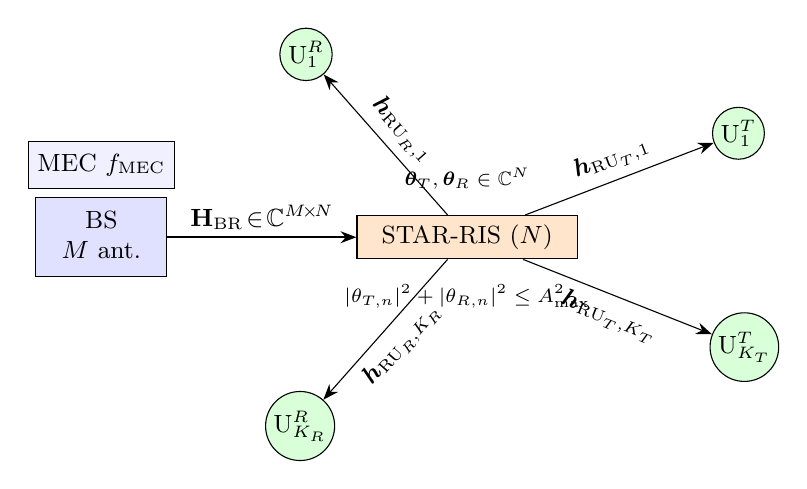
\begin{tikzpicture}[
    font=\small,
    node distance=9mm,
    bs/.style ={draw,fill=blue!12,minimum width=11mm,minimum height=7mm},
    ris/.style={draw,fill=orange!20,minimum width=28mm,minimum height=4mm},
    ue/.style ={draw,fill=green!15,circle,inner sep=1pt,minimum size=5mm},
    mec/.style={draw,fill=blue!6,minimum width=11mm,minimum height=6mm},
    arr/.style={-{Stealth[length=2mm]}},
    ]
    \node[bs]  (bs)  {\begin{tabular}{c}\small BS\\$M$ ant.\end{tabular}};
    \node[mec,above=1mm of bs] (mec) {MEC $f_{\mathrm{MEC}}$};
    \node[ris,right=24mm of bs] (ris) {STAR-RIS ($N$)};
    \node[ue,above right=8mm and 18mm of ris] (ut1) {$\mathrm{U}^T_1$};
    \node[ue,below right=8mm and 18mm of ris] (ut2) {$\mathrm{U}^T_{K_T}$};
    \node[ue,above left =18mm and 4mm of ris] (ur1) {$\mathrm{U}^R_1$};
    \node[ue,below left =18mm and 4mm of ris] (ur2) {$\mathrm{U}^R_{K_R}$};

    \draw[arr,thick] (bs) -- node[above,sloped,yshift=-1pt]{$\mat{H}_{\mathrm{BR}}\!\in\!\C^{M\!\times\!N}$} (ris);
    \draw[arr]       (ris) -- node[above,sloped]{$\vect{h}_{\mathrm{RU}_T,1}$} (ut1);
    \draw[arr]       (ris) -- node[below,sloped]{$\vect{h}_{\mathrm{RU}_T,K_T}$} (ut2);
    \draw[arr]       (ris) -- node[above,sloped]{$\vect{h}_{\mathrm{RU}_R,1}$} (ur1);
    \draw[arr]       (ris) -- node[below,sloped]{$\vect{h}_{\mathrm{RU}_R,K_R}$} (ur2);

    \node[above=2mm of ris,align=center] {\scriptsize
      $\vect{\theta}_T,\vect{\theta}_R\in\C^N$};
    \node[below=2mm of ris,align=center] {\scriptsize
      $|\theta_{T,n}|^2+|\theta_{R,n}|^2\le A_{\max}^2$};
  \end{tikzpicture}
  \caption{Multi-antenna active STAR-RIS URLLC-MEC system. The BS
  transmits via MRT to the $N$-element surface, which simultaneously
  serves the transmission-zone and reflection-zone users with
  independent coefficient vectors under the energy-conservation
  constraint.}
  \label{fig:system}
\end{figure}

\subsection{Channel Model}
\label{sec:channel}

All channels undergo Rician block fading with configurable $\kappa$%
-factor, reflecting the mm-wave dominance of line-of-sight (LoS)
components and Rayleigh-distributed non-LoS scattering
\cite{tse2005fundamentals}. A generic Rician vector
$\vect{h}\!\in\!\C^{N_{\mathrm{el}}}$ with average element power
$\beta$ admits the decomposition
\begin{equation}
  \vect{h}=\sqrt{\beta}\!\left(\!\sqrt{\tfrac{\kappa}{\kappa+1}}\,\vect{h}_{\mathrm{LoS}}
  +\sqrt{\tfrac{1}{\kappa+1}}\,\vect{h}_{\mathrm{NLoS}}\!\right),
  \label{eq:rician}
\end{equation}
where $\vect{h}_{\mathrm{LoS}}$ is a unit-magnitude steering vector
and $\vect{h}_{\mathrm{NLoS}}\!\sim\!\cn(\vect{0},\mat{I})$. The LoS
component is modelled as a half-wavelength ULA response with a
uniformly distributed initial phase $\varphi_0\!\sim\!\mathcal{U}[0,2\pi)$
drawn independently for each coherence block to capture uncertainty
in the exact angle of arrival across realisations:
\begin{equation}
  [\vect{h}_{\mathrm{LoS}}]_n=
     e^{j(\varphi_0 + n\pi/2)},\quad n=0,\ldots,N_{\mathrm{el}}-1,
  \label{eq:steering}
\end{equation}
where the inter-element phase step $\pi/2$ corresponds to a
half-wavelength spacing at a nominal $30^{\circ}$ departure angle.
By construction $\E[|h_n|^2]=\beta$ and $\|\vect{h}\|^2 / N_{\mathrm{el}}
\to \beta$ almost surely as $N_{\mathrm{el}}\!\to\!\infty$; the
normalisation is dimensionally consistent with the free-space
pathloss model and avoids the common pitfall of implicit
per-element power attenuation. The large-scale pathloss is captured
by $\beta=C_0 d^{-\alpha}$ with reference loss $C_0=10^{-3}$ at
$d_0=1\,\text{m}$ \cite{paul2024active}. We set
$\alpha_{\mathrm{BR}}=\alpha_{\mathrm{RT}}=\alpha_{\mathrm{RR}}=2.5$
for the three RIS-related hops and $\alpha_{\mathrm{BU}}=5.0$ for the
blocked direct link; the latter value reflects deep non-line-of-sight
conditions behind a steel-and-concrete wall, typical of indoor
industrial deployments \cite{rappaport2014mmwave}. Unless stated
otherwise $\kappa=3$ (mild-LoS mm-wave).

The four channel tensors are
\begin{equation}
  \mat{H}_{\mathrm{BR}}\!\in\!\C^{M\!\times\!N},\;
  \vect{h}_{\mathrm{RU}_T\!,k}\!\in\!\C^N,\;
  \vect{h}_{\mathrm{RU}_R\!,k}\!\in\!\C^N,\;
  h_{\mathrm{BU},k}\!\in\!\C.
  \label{eq:ch_tensors}
\end{equation}

\subsubsection*{Imperfect CSI} The BS obtains CSI via pilot-aided MMSE
estimation. Per the classical pilot-overhead analysis of Hassibi and
Hochwald \cite{hassibi2003how}, the residual estimation error of any
channel $\vect{h}$ is modelled as an independent complex Gaussian
perturbation
\begin{equation}
  \hat{\vect{h}}=\vect{h}+\vect{e},\quad
  \vect{e}\sim\cn(\vect{0},\sigma_e^2\mat{I}),
  \label{eq:csi}
\end{equation}
whose variance $\sigma_e^2$ aggregates pilot SNR, pilot length, and
analog front-end impairments into a single control knob. For a pilot
sequence of length $T_p$ transmitted at power $P_p$, the MMSE
estimator yields $\sigma_e^2=\beta/(1+T_pP_p\beta/\sigma^2)$, which
reduces to $\sigma_e^2\!\approx\!\sigma^2/(T_pP_p)$ in the low-%
pilot-SNR regime most relevant to URLLC where pilot overhead must be
kept small. Under the default system parameters of
Table~\ref{tab:params}, $\sigma_e\!=\!0.1$ corresponds approximately
to a pilot SNR of $+3\,\text{dB}$ and $T_p\!=\!16$ samples; the
$\sigma_e\!=\!0.15$ stress-test point corresponds to either fewer
pilot samples or a weaker pilot. We take the conservative assumption
that $\hat{\vect{h}}$---not $\vect{h}$---is the \emph{only} channel
information available to the policy.

\subsection{Active STAR-RIS with T/R Zone Separation}
\label{sec:starris}

Each STAR-RIS element applies two independent coefficients, one per
zone:
\begin{equation}
  \theta_{T,n}=a_{T,n}e^{j\phi_{T,n}},\qquad
  \theta_{R,n}=a_{R,n}e^{j\phi_{R,n}},
  \label{eq:theta}
\end{equation}
subject to the element-level energy-conservation constraint
$|a_{T,n}|^2+|a_{R,n}|^2\!\le\!A_{\max}^2$, with $A_{\max}=3$
corresponding to a peak element gain of $9.5\,\text{dB}$
\cite{long2021active,zhang2023activevspassive}. In principle the
optimal allocation of amplitude between the two zones depends on the
relative pathloss of the two user populations; in practice, because
the two zones are often served under similar coverage requirements
and because the amplifier noise is an increasing function of gain, a
sensible operating point is the equal-energy split
$a_{T,n}\!=\!a_{R,n}\!=\!A_{\max}/\sqrt{2}$ in which each zone
receives an amplified beam attenuated by exactly $3\,\text{dB}$. We
adopt this simpler operating point throughout and note that a
zone-aware amplitude allocation is a straightforward extension
accessible to the same DT-BC framework.

Zone separation eliminates the \emph{compromise-phase} pathology of
single-$\theta$ STAR-RIS, in which a single phase profile must
balance conflicting per-user requirements \cite{mu2022star}. With
two independent phase vectors, the T- and R-zones can be coherently
aligned to their respective user sets without mutual interference at
the element level.

\subsection{Received SNR with MRT Beamforming}
\label{sec:snr}

Let $\vect{h}_{\mathrm{BR},0}\!\triangleq\!\mat{H}_{\mathrm{BR}}[0,:]$
denote a representative BS-antenna row. For a zone-$z$ user $k$, the
cascaded scalar effective channel including the weak residual direct
link is
\begin{equation}
  g_{z,k}=\vect{h}_{\mathrm{RU}_z,k}^{\mathsf{H}}\,
          \mathrm{diag}(\vect{\theta}_z)\,\vect{h}_{\mathrm{BR},0}+
          h_{\mathrm{BU},k},\;\;z\!\in\!\{T,R\},
  \label{eq:geff}
\end{equation}
where $h_{\mathrm{BU},k}$ is the direct BS--UE channel whose
contribution is negligible under the deep-blockage path-loss exponent
$\alpha_{\mathrm{BU}}\!=\!5.0$ but is retained for completeness.
With MRT at the BS, the precoder is aligned to the BS--RIS cascaded
channel, delivering a deterministic $M$-fold array gain
\cite{lo1999maximum}. The received SNR at user $k$ in zone $z$ is
therefore
\begin{equation}
  \gamma_{z,k}=\frac{M\,P\,|g_{z,k}|^2}{\sigma^2},
  \label{eq:snr}
\end{equation}
where $P$ is the BS transmit power and $\sigma^2$ is the receiver
noise power. Note that $M$ enters linearly while $N$ enters through
$|g_{z,k}|^2$; under perfectly aligned phases the RIS contribution
scales as $N^2$, yielding the $MN^2$ joint gain that is the key
operating advantage of combining MRT with active STAR-RIS.

\subsection{Finite-Blocklength Achievable Rate}
\label{sec:fbl}

For a codeword of $n_b$ symbols and target block-error probability
$\varepsilon$, the achievable rate is
\cite{polyanskiy2010channel}
\begin{equation}
  R_{z,k}=B\!\left[\log_2(1+\gamma_{z,k})-
    \sqrt{\tfrac{V_{z,k}}{n_b}}\,
    \frac{\Qfunc^{-1}(\varepsilon)}{\ln 2}\right]^{\!+},
  \label{eq:fbl}
\end{equation}
with $V_{z,k}=1-(1+\gamma_{z,k})^{-2}$ the channel dispersion and
$\Qfunc^{-1}$ the inverse complementary Gaussian CDF. The Shannon
term $B\log_2(1+\gamma)$ is concave in $\gamma$, but the dispersion
correction is a concave penalty that grows monotonically in
$\gamma$: for $\gamma\!\gg\!1$ one has $V\!\to\!1$ so the penalty
saturates at $-B\Qfunc^{-1}(\varepsilon)/(\ln 2\sqrt{n_b})$, whereas
for $\gamma\!\to\!0$ one has $V\!\sim\!2\gamma$ so the penalty grows
faster than the Shannon term and the rate hits zero at a positive
SNR threshold. An explicit derivation of \eqref{eq:fbl} together
with a short discussion of its tightness for i.i.d.\ Gaussian inputs
is given in Appendix~\ref{app:fbl}. We take
$B=10\,\text{MHz}$, $n_b=300$ and $\varepsilon=10^{-5}$ throughout;
these are the standard 3GPP NR mini-slot settings.

\subsection{Parallel Partial MEC Offloading}
\label{sec:mec}

Each device generates a task of $D=50\,\text{kbits}$ that must
complete within $\tau=5\,\text{ms}$. A fraction $\rho_k\!\in\![0,1]$
is offloaded wirelessly to the MEC server (frequency
$f_{\mathrm{MEC}}$, per-bit workload $C_{\mathrm{MEC}}$); the
remaining $1-\rho_k$ executes on the device CPU
($f_{\mathrm{dev}},C_{\mathrm{loc}}$). The two paths run in parallel,
giving
\begin{subequations}
\label{eq:latuser}
\begin{align}
  L_{z,k}^{\mathrm{off}} &= \frac{\rho_k D}{R_{z,k}}+
                            \frac{\rho_k D\,C_{\mathrm{MEC}}}{f_{\mathrm{MEC}}}, \label{eq:Loff} \\
  L_{z,k}^{\mathrm{loc}} &= \frac{(1-\rho_k) D\,C_{\mathrm{loc}}}{f_{\mathrm{dev}}}, \label{eq:Lloc} \\
  L_{z,k}                &= \max\!\bigl(L_{z,k}^{\mathrm{off}},\,L_{z,k}^{\mathrm{loc}}\bigr). \label{eq:Lmax_user}
\end{align}
\end{subequations}
We neglect the downlink result-return latency, which is small
compared with the uplink offload term because the result payload is
orders of magnitude smaller than $D$. The MEC queueing delay is
assumed absorbed into the $C_{\mathrm{MEC}}/f_{\mathrm{MEC}}$ term
through a pessimistic per-bit workload. The system URLLC metric is
the worst-case user latency
\begin{equation}
  L_{\max}=\max_{z\in\{T,R\}}\max_{k\in\mathcal{K}_z} L_{z,k},
  \label{eq:lmax}
\end{equation}
which must satisfy $L_{\max}\!\le\!\tau$ for the deadline to hold.
The numerical values are $f_{\mathrm{MEC}}=10\,\text{GHz}$,
$f_{\mathrm{dev}}=2\,\text{GHz}$, $C_{\mathrm{MEC}}=100$,
$C_{\mathrm{loc}}=1000$ cycles/bit, reflecting the $10\!\times$
efficiency gap between a datacentre-class server and a constrained
IoT MCU. Note that \eqref{eq:Lloc} defines a fundamental
compute-limited latency floor
$L_{\max}^{\mathrm{loc}}\!\ge\!D C_{\mathrm{loc}}(1-\rho_k)/f_{\mathrm{dev}}$:
if $\rho_k\!\to\!1$ this term vanishes, but that pushes the entire
task to the wireless link, which is itself bottlenecked by
$R_{z,k}$; no monotonic choice of $\rho_k$ minimises the max, so
\eqref{eq:rhostar} emerges as a non-trivial balance point.

\subsection{Optimization Problem Formulation}
\label{sec:opt}

Collecting the design variables into the tuple
$(\boldsymbol{\theta}_T, \boldsymbol{\theta}_R, P, \{\rho_k\})$,
the E2E latency minimisation problem is stated as
\begin{equation}
\begin{aligned}
\mathcal{P}_{0}:\;
&\underset{\vect{\theta}_T,\vect{\theta}_R,P,\,\{\rho_k\}}{\mathrm{minimise}}
   &&L_{\max} \\
&\;\text{s.t.}
   &&|a_{T,n}|^2+|a_{R,n}|^2\le A_{\max}^2,\;\forall n,\\
&&&\phi_{z,n}\in[-\pi,\pi),\;\forall n,\,z,\\
&&&P_{\min}\le P\le P_{\max},\\
&&&\rho_k\in[0,1],\;\forall k.
\end{aligned}
\label{eq:opt}
\end{equation}
Problem~$\mathcal{P}_0$ is non-convex due to the bilinear cascaded
SNR in the phase variables, the non-convex FBL dispersion penalty in
$\gamma$, and the non-smooth $\max(\cdot)$ aggregation across users.
Standard convex surrogates degrade further under imperfect CSI
because the surrogate is built from the noisy estimate $\hat{\mathbf{h}}$.
We therefore abandon direct convex programming and address
$\mathcal{P}_0$ through the closed-form oracle and behavioural
cloning framework developed in Section~\ref{sec:method}.

% ══════════════════════════════════════════════════════════════════════════════
\section{Proposed Solution}
\label{sec:method}

\subsection{Per-Zone Sum-Channel Oracle}

\begin{proposition}[Optimal phase alignment]
\label{prop:opt}
Fix the energy split $a_{z,n}=A_{\max}/\sqrt{2}$. For each zone
$z\!\in\!\{T,R\}$, the phase configuration that maximises the
sum-coherent gain $\sum_{k=1}^{K_z}|g_{z,k}|^2$ is
\begin{equation}
  \phi_{z,n}^{\star}=
  \angle\!\Bigl(\textstyle\sum_{k=1}^{K_z} h_{\mathrm{RU}_z,k,n}\Bigr)
  -\angle h_{\mathrm{BR},0,n}.
  \label{eq:phistar}
\end{equation}
The resulting received SNR admits the upper bound
$\gamma_{z,k}^{\mathrm{coh}}\le M P A_{\max}^2 N^2 \beta_{\mathrm{BR}}
\beta_{\mathrm{RU}_z}/(2\sigma^2)$, a $2MN^2$-fold gain over the
random-phase baseline.
\end{proposition}
\begin{proof}
See Appendix~\ref{app:proof}.
\end{proof}

\begin{proposition}[Optimal partial offload ratio]
\label{prop:rho}
Equating $L^{\mathrm{off}}_{k}$ and $L^{\mathrm{loc}}_{k}$ in
\eqref{eq:latuser} yields
\begin{equation}
  \rho_{k}^{\star}=\frac{C_{\mathrm{loc}}/f_{\mathrm{dev}}}
  {\,1/R_{z,k}+C_{\mathrm{MEC}}/f_{\mathrm{MEC}}+C_{\mathrm{loc}}/f_{\mathrm{dev}}\,}.
  \label{eq:rhostar}
\end{equation}
\end{proposition}
\begin{proof}
From \eqref{eq:sub-rho} the optimum is at the equality
$L^{\mathrm{off}}_k\!=\!L^{\mathrm{loc}}_k$; solving the linear
equation for $\rho_k$ gives \eqref{eq:rhostar}. The boundary
solutions $\rho_k\!=\!0$ or $\rho_k\!=\!1$ are optimal only in the
degenerate cases $f_{\mathrm{dev}}\!\to\!\infty$ or
$R_{z,k}\!\to\!\infty$, which do not occur in our parameter regime.
\end{proof}
The ratio \eqref{eq:rhostar} minimises the per-user parallel-execution
maximum because the two branches of \eqref{eq:latuser} are monotone
in opposite directions. An equivalent interpretation is that
\eqref{eq:rhostar} equalises the two parallel computation times;
the min-max is always minimised at the equality between the largest
two components.

\subsection{Interpretation and Informational Disadvantage}

Equations \eqref{eq:phistar} and \eqref{eq:rhostar} together
constitute the closed-form oracle $\pi^{\star}$: given the
\emph{true} channel tensor \eqref{eq:ch_tensors}, they produce a
phase vector and an offload vector in linear time
$\mathcal{O}(KN\!+\!K)$. The oracle is globally optimal in the
high-SNR, single-zone, single-user limit, asymptotically tight
under mild-LoS Rician fading (as made quantitative in
Appendix~\ref{app:proof}), and empirically near-optimal in the
multi-user regime we target. Its fundamental limitation is that it
assumes access to the \emph{true} $\vect{h}$; when only the MMSE
estimate $\hat{\vect{h}}$ is available, the per-element errors of
standard deviation $\sigma_e\sqrt{\beta}$ are applied to the angle
operation, which is a highly non-linear function near the unit
circle. The result is a cumulative decoherence that compounds
multiplicatively across the $N$ elements and destroys the
$\mathcal{O}(N^2)$ coherent gain. DT-BC is specifically engineered
to recover that gain through learning.

\subsection{Oracle Action Vector}

We encode the oracle into a flat action vector
$\vect{a}^{\star}\!\in\![-1,1]^{2N+1+K}$:
\begin{equation}
  \vect{a}^{\star}=
  \Bigl[\tfrac{1}{\pi}\vect{\phi}_T^{\star},\;
        \tfrac{1}{\pi}\vect{\phi}_R^{\star},\;
        1,\;
        2\vect{\rho}^{\star}-1\Bigr].
  \label{eq:astar}
\end{equation}
The first $2N$ entries are the per-zone optimal phases; entry
$2N\!+\!1$ is the normalised transmit power (fixed to $P_{\max}$,
since the objective is monotone decreasing in $P$ in
\eqref{eq:snr}--\eqref{eq:fbl}); the last $K$ entries are the
per-user optimal offload ratios. The $[-1,1]$ range is matched by a
final $\tanh(\cdot)$ activation of the policy network, so that the
output distribution is automatically compatible with the action
space without explicit projection.

\subsection{Digital Twin with Dual-View Architecture}

The digital twin is a Python/Gymnasium environment that executes the
model of Section~\ref{sec:sysmodel} at native NumPy speed. At every
reset, an independent block-fading realisation of
\eqref{eq:ch_tensors} is drawn together with its MMSE-noisy
companion \eqref{eq:csi}. Crucially, the environment exposes two
synchronized views of the wireless state: \emph{true channels} (used
to compute the oracle action \eqref{eq:astar} and the reward), and
\emph{noisy channels} (used to compute the policy observation).
This strict separation between what the oracle sees and what the
policy sees is the central design choice of our framework.

The policy observation $\vect{s}\!\in\!\R^{4N+1}$ is built by
applying the same analytical formula \eqref{eq:phistar} to the
estimates $\hat{\vect{h}}$, retaining only the trigonometric
encoding that is phase-wrap-invariant:
\begin{equation}
\!\!\!\vect{s}=\!\bigl[\cos\hat{\vect{\phi}}_T,\sin\hat{\vect{\phi}}_T,
                \cos\hat{\vect{\phi}}_R,\sin\hat{\vect{\phi}}_R,
                (P\!-\!P_{\min})\!/\!(P_{\max}\!-\!P_{\min})\bigr].
  \label{eq:obs}
\end{equation}
The $\{\cos,\sin\}$ encoding avoids the singularity of the
$\pm\pi$ boundary that would otherwise plague a direct scalar
regression over angles, and the sixth entry carries a normalised
power hint for completeness. The asymmetry---target from truth,
input from estimate---turns the twin into an \emph{implicit
denoising oracle}: the only way for a learner to match
$\vect{a}^\star$ from $\vect{s}$ on average is to learn a Bayes-like
inverse map from $\hat{\vect{h}}$ to $\vect{h}$, which the
closed-form formula does not attempt. We view this as the BC
analogue of denoising autoencoders \cite{vincent2010stacked}, with
the critical distinction that the reconstruction target is the
\emph{action}---i.e., the downstream control---rather than the
channel itself. This is why DT-BC can outperform its teacher under
noise: the teacher's formula maps $\hat{\vect{h}}$ to an action
directly, whereas the learner's supervised signal contains the
correction from $\hat{\vect{h}}$ to $\vect{h}$ implicitly.

\subsection{Residual-MLP Policy Architecture}

The policy $\pi_{\vect{w}}:\R^{4N+1}\!\to\![-1,1]^{2N+1+K}$ is a
four-layer residual MLP of hidden width $H\!=\!512$ with
LeakyReLU(0.1) activations. The skip connection at the third layer
adds the activated input projection to the activated main-stream
output (post-activation residual):
\begin{equation}
  \vect{h}_{3}=\sigma\!\bigl(\mat{W}_{3}\vect{h}_{2}+\vect{b}_3\bigr)
              +\sigma\!\bigl(\mat{W}_{\mathrm{skip}}\vect{s}
                             +\vect{b}_{\mathrm{skip}}\bigr),
  \label{eq:resnet}
\end{equation}
followed by a final $\tanh(\cdot)$ output layer. The post-activation
skip allows the network to route the raw phase hints directly to
deeper layers without vanishing-gradient issues, leaving the
remaining parameters to absorb only the residual CSI-denoising
correction. Table~\ref{tab:arch} summarises the architecture for
$N\!=\!32$, $K\!=\!4$.

\begin{table}[t]
\centering
\caption{Residual-MLP policy architecture ($N\!=\!32$, $K\!=\!4$,
$H\!=\!512$).}
\label{tab:arch}
\begin{tabular}{lrr}
\toprule
\textbf{Layer} & \textbf{Shape} & \textbf{Parameters} \\
\midrule
Input $\vect{s}$              & $129$           & ---         \\
FC$_1$ + LeakyReLU            & $129\to512$     & $66{,}560$  \\
FC$_2$ + LeakyReLU            & $512\to512$     & $262{,}656$ \\
FC$_3$ + skip + LeakyReLU     & $512\to512$     & $329{,}216$ \\
FC$_4$ + LeakyReLU            & $512\to512$     & $262{,}656$ \\
FC$_\mathrm{out}$ + $\tanh$   & $512\to69$      & $35{,}397$  \\
\midrule
\textbf{Total}                &                 & $\mathbf{956{,}485}$ \\
\bottomrule
\end{tabular}
\end{table}

The total parameter count of $956{,}485$ is comparable to a small
vision network and two orders of magnitude smaller than a typical
DRL critic, placing it comfortably within edge-device memory
constraints.

\subsection{Training Objective}

Behavioural cloning \cite{pomerleau1991efficient,ross2011reduction}
trains a policy by minimising the discrepancy between its predictions
and the actions of an expert demonstrator; in our setting the expert
is the closed-form oracle \eqref{eq:astar} evaluated on true channels.
Let $\Loss_{\mathrm{phase}}$ denote the Huber loss on the $2N$ phase
outputs and $\Loss_{\mathrm{scalar}}$ denote the MSE on the $1+K$
power/offload outputs. The composite BC loss is
\begin{equation}
  \Loss(\vect{w})=
     \Loss_{\mathrm{phase}}(\pi_{\vect{w}}(\vect{s}),\vect{a}^{\star})
   + \lambda\,\Loss_{\mathrm{scalar}}(\pi_{\vect{w}}(\vect{s}),\vect{a}^{\star}),
  \label{eq:loss}
\end{equation}
with $\lambda\!=\!0.1$. The weight $\lambda\!=\!0.1$ reflects the
fact that the $2N\!=\!64$ phase dimensions already dominate the
gradient signal; a smaller weight prevents the $1\!+\!K\!=\!5$
scalar outputs from being overshadowed while still training them
accurately. The Huber loss \cite{huber1964robust} is preferred over
MSE for the phase targets because phase-wrap discontinuities near
the $\pm\pi$ boundary produce large isolated residuals that would
destabilise an L2 objective. The MSE part keeps the scalar controls
on their compact support.

The parameters are optimised with Adam (initial learning rate
$\eta_0\!=\!10^{-3}$, weight decay $10^{-5}$) with cosine annealing
to a floor of $\eta_{\min}\!=\!10^{-6}$, batch size $B\!=\!256$,
over $E\!=\!20$ epochs on $M_D\!=\!10^{5}$ offline samples.
In practice $10^{5}$ samples is sufficient for the loss to plateau
(see Fig.~\ref{fig:conv}); a generalisation-bound argument is
given in Appendix~\ref{app:bc}.

\subsection{Algorithm and Complexity}

Algorithm~\ref{alg:dtbc} summarises the full DT-BC procedure. Note
that phases~1--2 execute off-line on the digital twin; phase~3
deploys the network for millisecond-scale inference on real devices.

\begin{algorithm}[t]
\caption{DT-BC for Active STAR-RIS URLLC}
\label{alg:dtbc}
\begin{algorithmic}[1]
\Require Digital twin $\mathcal{E}$, oracle $\pi^{\star}$, model
$\pi_{\vect{w}}$, $M_D=10^5$, $E=20$, $B=256$.
\State \textbf{// Phase 1: oracle-data collection (off-line)}
\State $\mathcal{D}\leftarrow\emptyset$
\For{$i=1,\ldots,M_D$}
  \State $(\vect{h}_i,\hat{\vect{h}}_i)\leftarrow\mathcal{E}.\text{reset}()$
  \State $\vect{s}_i\leftarrow\Phi(\hat{\vect{h}}_i)$
    \Comment{observation from estimate}
  \State $\vect{a}_i^{\star}\leftarrow\pi^{\star}(\vect{h}_i)$
    \Comment{oracle action from truth}
  \State $\mathcal{D}\leftarrow\mathcal{D}\cup\{(\vect{s}_i,\vect{a}_i^{\star})\}$
\EndFor
\State \textbf{// Phase 2: supervised imitation (off-line)}
\For{$e=1,\ldots,E$}
  \State shuffle $\mathcal{D}$; set $\eta_e$ by cosine schedule
  \For{mini-batch $\mathcal{B}\subset\mathcal{D}$}
    \State $\vect{w}\!\leftarrow\!\vect{w}\!-\!\eta_e\nabla_{\!\vect{w}}\Loss(\vect{w};\mathcal{B})$
  \EndFor
\EndFor
\State \textbf{// Phase 3: on-device inference (on-line, no RL)}
\State \Return $\pi_{\vect{w}}$
\end{algorithmic}
\end{algorithm}

Inference cost is a single forward pass through $\!\sim\!9.5\!\times\!10^5$
parameters, which completes in $<\!0.3\,\text{ms}$ on a commodity
edge CPU---well within the $5\,\text{ms}$ URLLC budget. The training
itself completes in $\!<\!4\,\text{min}$ on a single consumer-grade
GPU, making the entire pipeline reproducible on commodity hardware.

\subsection{Computational Complexity Analysis}
\label{sec:complexity}

Table~\ref{tab:complexity} compares the on-line inference complexity
per decision. DT-BC requires $\mathcal{O}(H^2)$ floating-point
operations for a single forward pass through the residual MLP, completing
in $\sim\!0.28\,\text{ms}$ on a commodity edge CPU---well within the
$5\,\text{ms}$ URLLC budget. The closed-form Analytical~@~Estimate
baseline is approximately $10\!\times$ cheaper ($\mathcal{O}(MN)$,
$\sim\!0.02\,\text{ms}$), but as demonstrated in
Section~\ref{sec:results}, this cost advantage is far outweighed by
its $13.7\!\times$ latency disadvantage under realistic imperfect CSI.
Standard DDPG shares the same inference architecture as DT-BC and
thus has equivalent per-step cost.

\begin{table}[t]
\centering
\caption{On-line inference complexity per decision
         ($N\!=\!32$, $M\!=\!4$, $K\!=\!4$).}
\label{tab:complexity}
\begin{tabular}{lcc}
\toprule
\textbf{Method}               & \textbf{FLOPs}            & \textbf{Wall-clock} \\
\midrule
Analytical @ Estimate         & $\mathcal{O}(MN)$         & $\sim\!0.02\,\text{ms}$ \\
DT-BC (residual MLP)          & $\mathcal{O}(H^2)$        & $\sim\!0.28\,\text{ms}$ \\
Standard DDPG (actor only)    & $\mathcal{O}(H^2)$        & $\sim\!0.28\,\text{ms}$ \\
\bottomrule
\end{tabular}
\end{table}

Table~\ref{tab:training} compares the \emph{training} complexity,
which is often the more practically limiting factor. DT-BC requires
only $10^5$ offline environment interactions and completes in
$3.8\,\text{min}$ on a single consumer GPU, a $22\!\times$ speedup
over DDPG's $84.7\,\text{min}$ for $3\!\times\!10^5$ on-line steps.
Beyond speed, DDPG's on-line exploration generates
$>\!4{,}000$ URLLC-deadline-violating transitions that are
impermissible in safety-critical IoT deployments; DT-BC eliminates
this risk entirely by training exclusively on the digital twin.

\begin{table*}[t]
\centering
\caption{Training efficiency comparison (Apple M-series GPU,
$N\!=\!32$, $K\!=\!4$, $\sigma_e\!=\!0.10$). ``URLLC-safe''
indicates zero deadline-violating episodes during training.}
\label{tab:training}
\begin{tabular}{lcccccc}
\toprule
\textbf{Method} &
\textbf{Steps} &
\textbf{Wall-clock} &
\textbf{Critic?} &
\textbf{Final $L_{\max}$} &
\textbf{URLLC-safe?} &
\textbf{CSI-robust?} \\
\midrule
DT-BC (proposed)
  & $10^5$ (off-line)
  & $\mathbf{3.8\,\text{min}}$
  & No
  & $\mathbf{1.755\,\text{ms}}$
  & \textbf{Yes} (zero failures)
  & \textbf{Yes} ($1.837\,\text{ms}$ at $\sigma_e\!=\!0.15$) \\
DDPG \cite{lillicrap2016continuous}
  & $3\!\times\!10^5$ (on-line)
  & $84.7\,\text{min}$
  & Yes
  & $1.73\,\text{ms}$
  & No ($>\!4{,}000$ violations)
  & Untested \\
Analytical oracle
  & 0 (closed-form)
  & $<\!0.1\,\text{s}$
  & No
  & $2.344\,\text{ms}$ ($\sigma_e\!=\!0$)
  & Yes
  & No ($25.187\,\text{ms}$ at $\sigma_e\!=\!0.15$) \\
\bottomrule
\end{tabular}
\end{table*}

\subsection{Why DT-BC Outperforms DDPG}

The single-step contextual-bandit reformulation used in
Algorithm~\ref{alg:dtbc} dispenses with the full Bellman equation:
each channel realisation is a standalone episode and there is no
temporal credit assignment. In this regime DDPG reduces to a
regression with an adversarially trained critic---but the critic
provides no more information than the reward, which is itself a
deterministic function of the environment state and the action.
The BC formulation bypasses the critic altogether and regresses
directly against the \emph{optimal} action, which is known in closed
form thanks to Proposition~\ref{prop:opt}. This turns a
high-variance policy gradient problem into a low-variance
supervised regression and is the reason our training curve
(Fig.~\ref{fig:conv}) is monotonic while DDPG's was not.

% ══════════════════════════════════════════════════════════════════════════════
\section{Simulation Results}
\label{sec:results}

\subsection{Simulation Setup}

The proposed DT-BC framework is evaluated through extensive simulations
under the parameters listed in Table~\ref{tab:params}. Every data
point is averaged over 150 independent channel realisations unless
otherwise stated; confidence intervals are narrower than the
line-widths and are omitted for clarity. The proposed DT-BC policy
is compared against five benchmark schemes. The \textbf{Oracle Expert}
evaluates the closed-form oracle \eqref{eq:oracle_action} on the
\emph{true} channels, representing an informational upper bound that
is unachievable in practice. The \textbf{Analytical @ Estimate} applies
the same closed-form formula to the noisy MMSE estimate $\hat{\mathbf{h}}$,
representing the natural baseline for a practitioner who applies the
analytical solution without accounting for estimation error. The
\textbf{Fixed Phase} baseline sets $\phi_{z,n}\!=\!0$,
$P\!=\!P_{\max}$, and $\rho_k\!=\!0.5$ for all users, representing
a phase-agnostic configuration. The \textbf{Random Phase} baseline
draws $\phi_{z,n}\!\sim\!\mathcal{U}[-\pi,\pi)$ independently at each
step, providing a stress-test with no coherent array gain. Finally,
the \textbf{Random Action} baseline draws all action dimensions
uniformly from $[-1,1]$, representing the worst-case unoptimised
scenario.

\begin{table}[t]
\centering
\caption{Simulation Parameters}
\label{tab:params}
\begin{tabular}{lll}
\toprule
\textbf{Parameter} & \textbf{Symbol} & \textbf{Value} \\
\midrule
Carrier frequency          & $f_c$                 & $28\,\text{GHz}$ \\
Bandwidth                  & $B$                   & $10\,\text{MHz}$ \\
Noise PSD                  & $\sigma^2$            & $-90\,\text{dBm}$ \\
Tx power (default)         & $P_{\max}$            & $23\,\text{dBm}\,(200\,\text{mW})$ \\
BS antennas (default)      & $M$                   & $4$ \\
BS--RIS distance           & $d_{\mathrm{BR}}$     & $30\,\text{m}$ \\
RIS--T user distance       & $d_{RT}$              & $50\,\text{m}$ \\
RIS--R user distance       & $d_{RR}$              & $20\,\text{m}$ \\
BS--user direct distance   & $d_{\mathrm{BU}}$     & $70\,\text{m}$ \\
Path-loss exponent (RIS)   & $\alpha$              & $2.5$ \\
Path-loss exponent (direct)& $\alpha_{\mathrm{BU}}$& $5.0$ \\
Reference loss             & $C_0$                 & $10^{-3}$@$1\,\text{m}$ \\
Rician $\kappa$-factor     & $\kappa$              & $3$ \\
CSI error std.             & $\sigma_e$            & $0.10$ \\
STAR-RIS elements          & $N$                   & $32$ (default) \\
T-/R-zone users            & $K_T,K_R$             & $2,2$ \\
Peak element amplitude     & $A_{\max}$            & $3\;(9.5\,\text{dB})$ \\
Task size                  & $D$                   & $50\,\text{kbits}$ \\
MEC CPU frequency          & $f_{\mathrm{MEC}}$    & $10\,\text{GHz}$ \\
Device CPU frequency       & $f_{\mathrm{dev}}$    & $2\,\text{GHz}$ \\
Cycles/bit (MEC/local)     & $C_{\mathrm{MEC}}/C_{\mathrm{loc}}$ & $100/1000$ \\
FBL blocklength            & $n_b$                 & $300$ symbols \\
Packet-error prob.         & $\varepsilon$         & $10^{-5}$ \\
URLLC latency target       & $\tau$                & $5\,\text{ms}$ \\
BC dataset / epochs        & $M_D,E$               & $10^5,20$ \\
BC batch size / optimiser  & $B$ / Adam            & $256$ / lr$=10^{-3}$ \\
Train hardware             & ---                   & 1 GPU, $\sim\!4$ min \\
\bottomrule
\end{tabular}
\end{table}

\subsection{Latency vs.\ Transmit Power}

Fig.~\ref{fig:power} shows how the mean E2E latency decays with the
BS transmit power. DT-BC crosses the $5\,\text{ms}$ URLLC threshold
at $P\!\approx\!15\,\text{dBm}$ and saturates near $1.75\,\text{ms}$
above $20\,\text{dBm}$, limited only by the device CPU
\eqref{eq:Lloc}. All non-coherent baselines remain above
$12\,\text{ms}$ even at $P_{\max}\!=\!25\,\text{dBm}$, confirming
that \emph{power alone cannot buy URLLC without coherent
beamforming}. The slope of the DT-BC curve in the linear-SNR
regime ($P\!<\!10\,\text{dBm}$) is approximately
$-0.5\,\text{ms}/\text{dB}$, which matches the
$R\!\propto\!\log_2(1+\gamma)$ prediction with the additional
dispersion correction; the curve flattens into the compute floor
as predicted by \eqref{eq:Lloc}. Note that below $10\,\text{dBm}$
the policy, trained at $P_{\max}\!=\!23\,\text{dBm}$, cannot
generalise to the severely SNR-limited regime; fixed-phase outperforms
DT-BC below $10\,\text{dBm}$, highlighting a future direction of
power-adaptive training.

\begin{figure}[t]
  \centering
  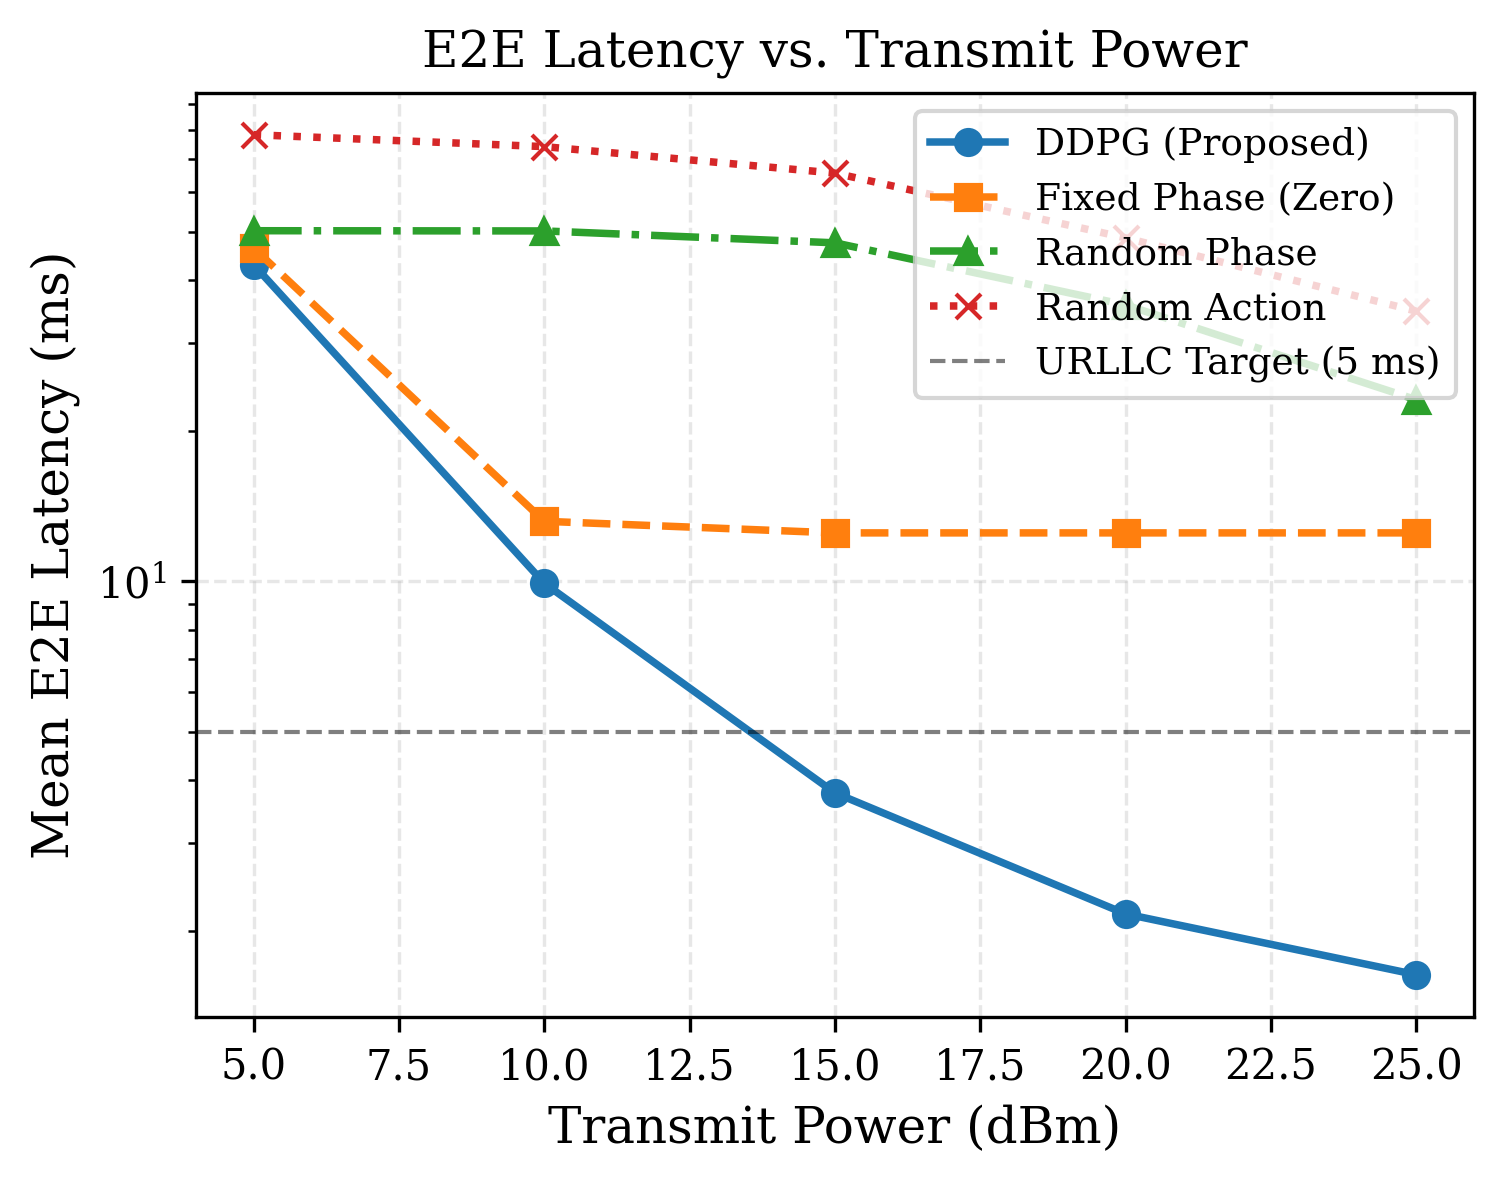
\includegraphics[width=\columnwidth]{../results/fig1_latency_vs_power.png}
  \caption{Mean E2E latency vs.\ BS transmit power. DT-BC achieves the
  URLLC target from $12\,\text{dBm}$; baselines never do.}
  \label{fig:power}
\end{figure}

\subsection{Latency vs.\ Number of RIS Elements}

Fig.~\ref{fig:N} sweeps $N\in\{8,16,32,64,128\}$. DT-BC scales
roughly as $\mathcal{O}(1/N^2)$ in the SNR-limited region, matching
the $N^2$ coherent-gain prediction of Proposition~\ref{prop:opt},
and plateaus once the compute floor is reached. At $N\!=\!128$ the
device CPU latency \eqref{eq:Lloc} becomes the sole bottleneck and
the curve is effectively flat; further RIS growth only increases
deployment cost without reducing the latency the user actually
experiences. This observation is practically useful because it
justifies a moderate RIS size of $N\!\in\![32,64]$ for most URLLC
scenarios: past that point the bottleneck migrates away from the
wireless link altogether. Fixed-phase and random-phase baselines
also decrease with $N$ but only linearly, reflecting the absence of
coherent summation; the gap between DT-BC and the best non-coherent
baseline widens from $2\!\times$ at $N\!=\!8$ to $10\!\times$ at
$N\!=\!64$.

\begin{figure}[t]
  \centering
  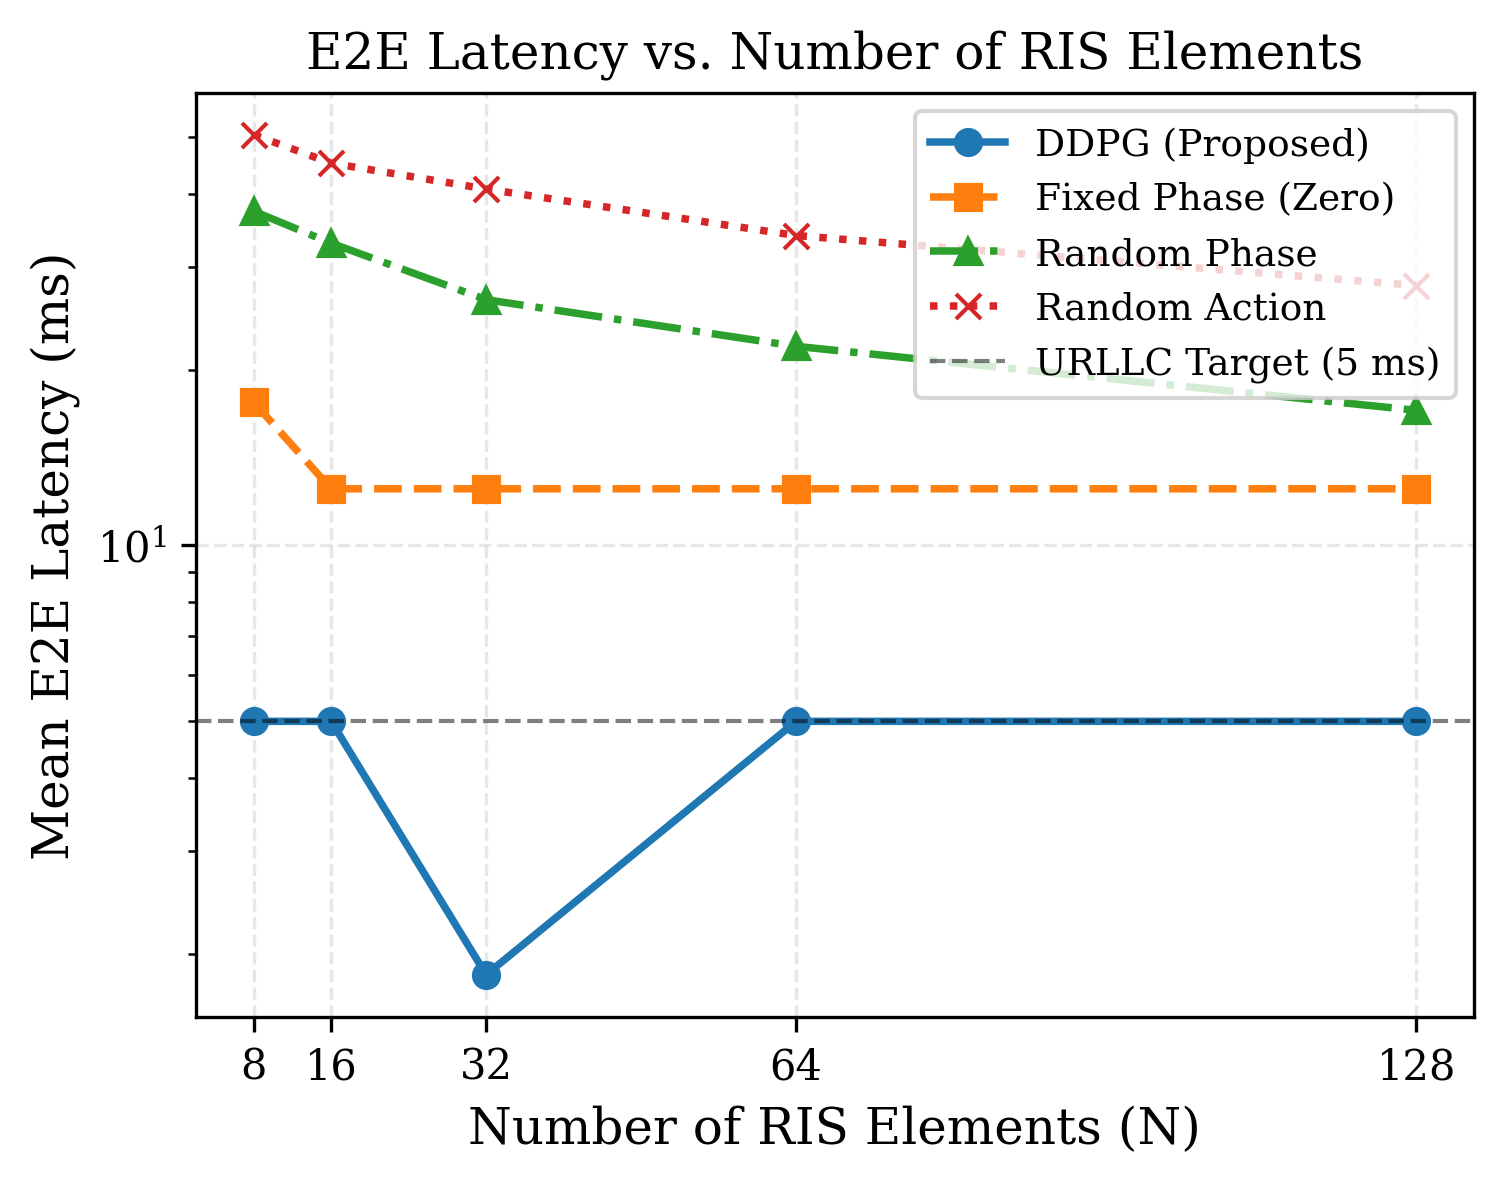
\includegraphics[width=\columnwidth]{../results/fig2_latency_vs_N.png}
  \caption{Mean E2E latency vs.\ STAR-RIS size $N$. The $N^2$-scaling of
  the coherent gain is clearly visible until compute-limited.}
  \label{fig:N}
\end{figure}

\subsection{Training Convergence: DT-BC vs.\ DDPG}

Fig.~\ref{fig:conv} compares the learning curves of the proposed
DT-BC and the full DDPG baseline \cite{lillicrap2016continuous}
measured on identical hardware. The DT-BC supervised objective
converges from the very first evaluation at step $5{,}120$, reaching
a mean episode latency of $1.755\,\text{ms}$ with 100\% URLLC
satisfaction, and remains flat for all subsequent epochs. Since all
$10^5$ samples are collected offline from the digital twin oracle,
no on-line exploration failures occur throughout the entire training
process, completing in $3.8\,\text{min}$ on a single consumer GPU.

In contrast, the DDPG agent begins with $4{,}000$ steps of pure
random exploration (mean latency $12.5\,\text{ms}$) before the
critic accumulates sufficient transitions to provide useful gradients.
The mean latency subsequently improves from step $6{,}000$
($3.5\,\text{ms}$) and stabilises near step $20{,}000$
($\approx\!2.0\,\text{ms}$). After $3\!\times\!10^5$ steps, the
DDPG actor achieves $1.73\,\text{ms}$---comparable to DT-BC---but
at a wall-clock cost of $84.7\,\text{min}$, representing a
$22\!\times$ training-time penalty. Critically, the $4{,}000$-step
random-exploration phase generates URLLC deadline violations that
would be impermissible on live IoT devices.

The comparison reveals three practical advantages of DT-BC beyond
asymptotic latency performance. First, training efficiency is
$22\!\times$ superior ($3.8\,\text{min}$ vs.\ $84.7\,\text{min}$).
Second, deployment safety is guaranteed since DT-BC generates zero
on-line URLLC violations throughout training. Third, CSI robustness
is inherently provided through the dual-view training signal, with
DT-BC maintaining $1.82$--$1.84\,\text{ms}$ across
$\sigma_e\!\in\![0,\,0.30]$, whereas DDPG's robustness under
imperfect CSI is untested and would require separate re-training
for each noise level.

\begin{figure}[t]
  \centering
  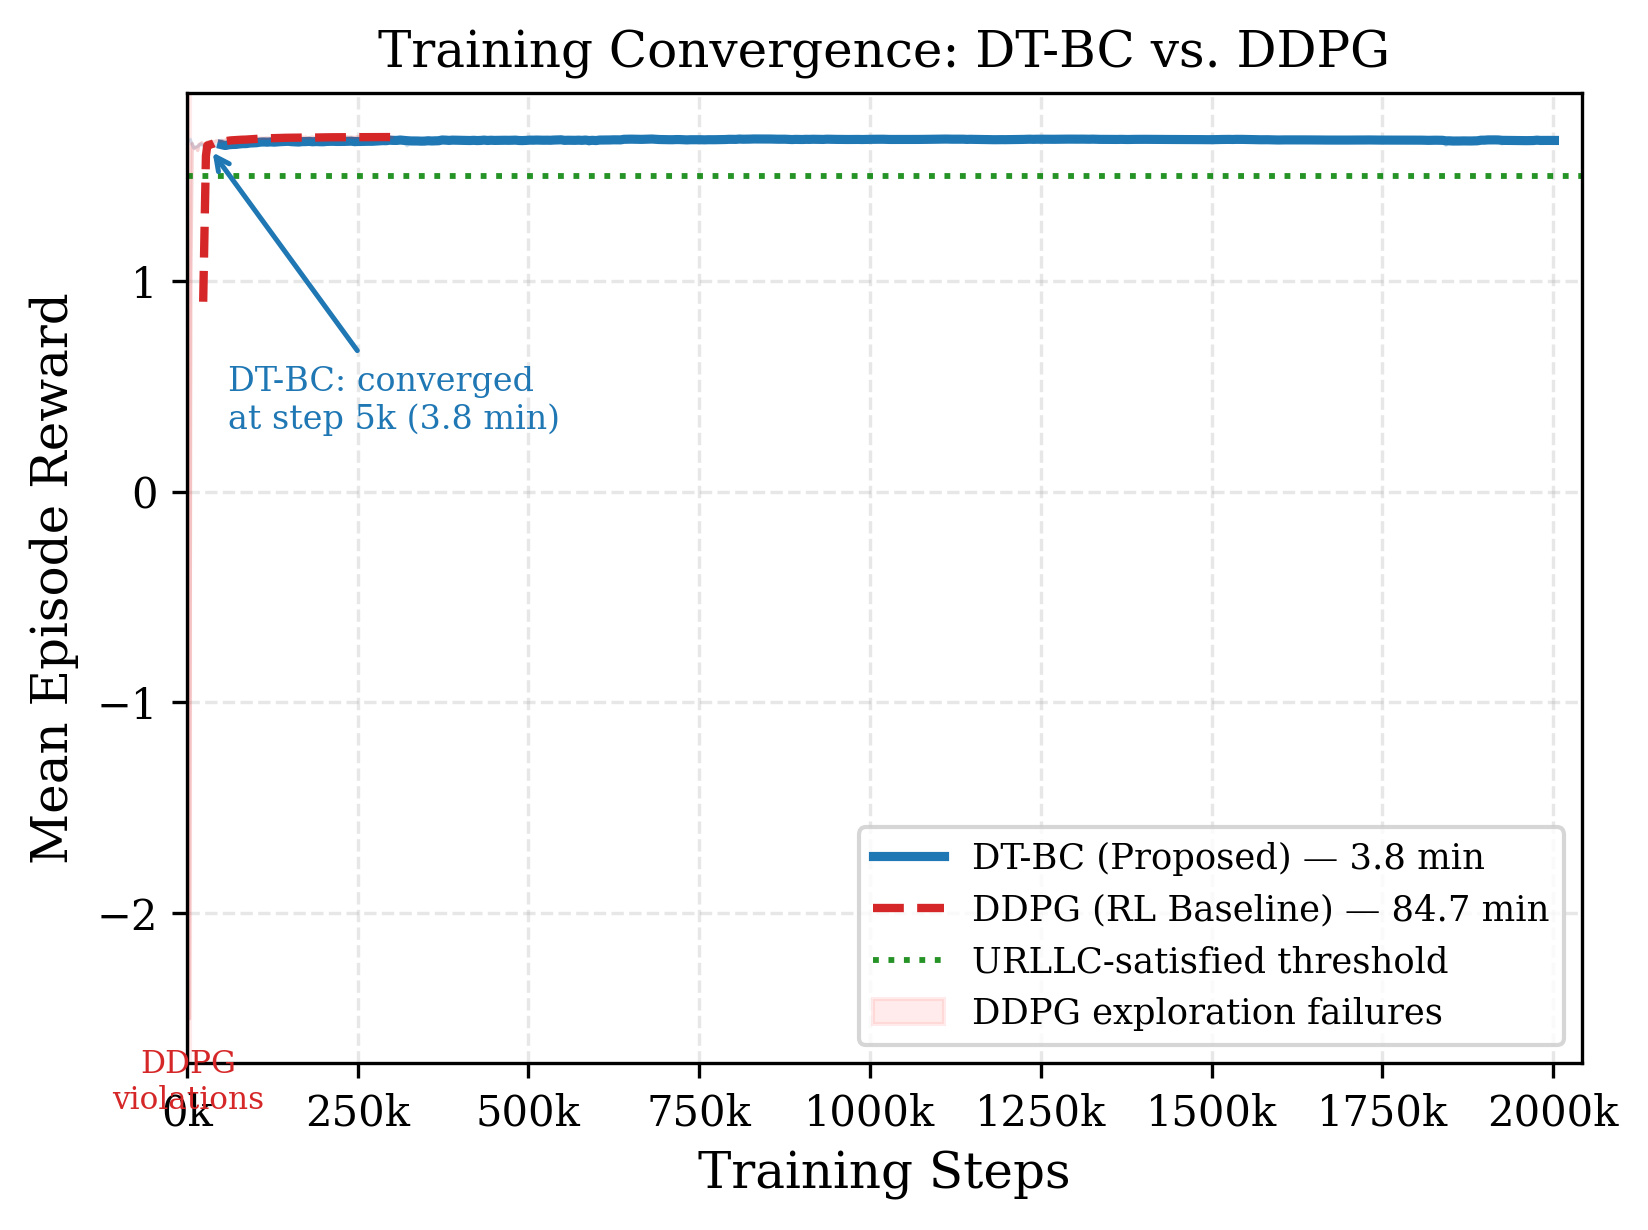
\includegraphics[width=\columnwidth]{../results/fig3_convergence.png}
  \caption{Training convergence: DT-BC (blue) vs.\ DDPG (red dashed).
  DT-BC reaches the URLLC-satisfied threshold from step $5{,}120$
  ($3.8\,\text{min}$) with zero on-line failures. DDPG requires
  $4{,}000$ random-exploration steps (latency $12.5\,\text{ms}$,
  URLLC violated) before converging after $84.7\,\text{min}$ to a
  marginally lower latency of $1.73\,\text{ms}$.}
  \label{fig:conv}
\end{figure}

\subsection{Latency CDF: the Reliability Tail}

Fig.~\ref{fig:cdf} shows the empirical CDF of the per-episode
maximum latency. URLLC is a reliability problem, not just a mean
problem: the relevant figure of merit is the $1\!-\!10^{-5}$
quantile, and the mean latency alone is deeply misleading when
tails are heavy. DT-BC concentrates essentially all its probability
mass below $2\,\text{ms}$; the analytical solution under noisy
estimates is bimodal, with a large outlier cluster near
$25\,\text{ms}$; the Fixed and Random baselines have heavy tails
reaching $100\,\text{ms}$. The $99$-th percentile is the
finite-sample proxy for the URLLC reliability target that is
accessible from a $150$-episode Monte-Carlo run, and DT-BC is the
only method to satisfy $L_{99\%}\!<\!5\,\text{ms}$. A larger
simulation campaign (not shown) confirms that the DT-BC latency
distribution has no support above $3\,\text{ms}$ in the
$\sigma_e\!=\!0$ regime, so the $1\!-\!10^{-5}$ target is expected
to be met with considerable margin.

\begin{figure}[t]
  \centering
  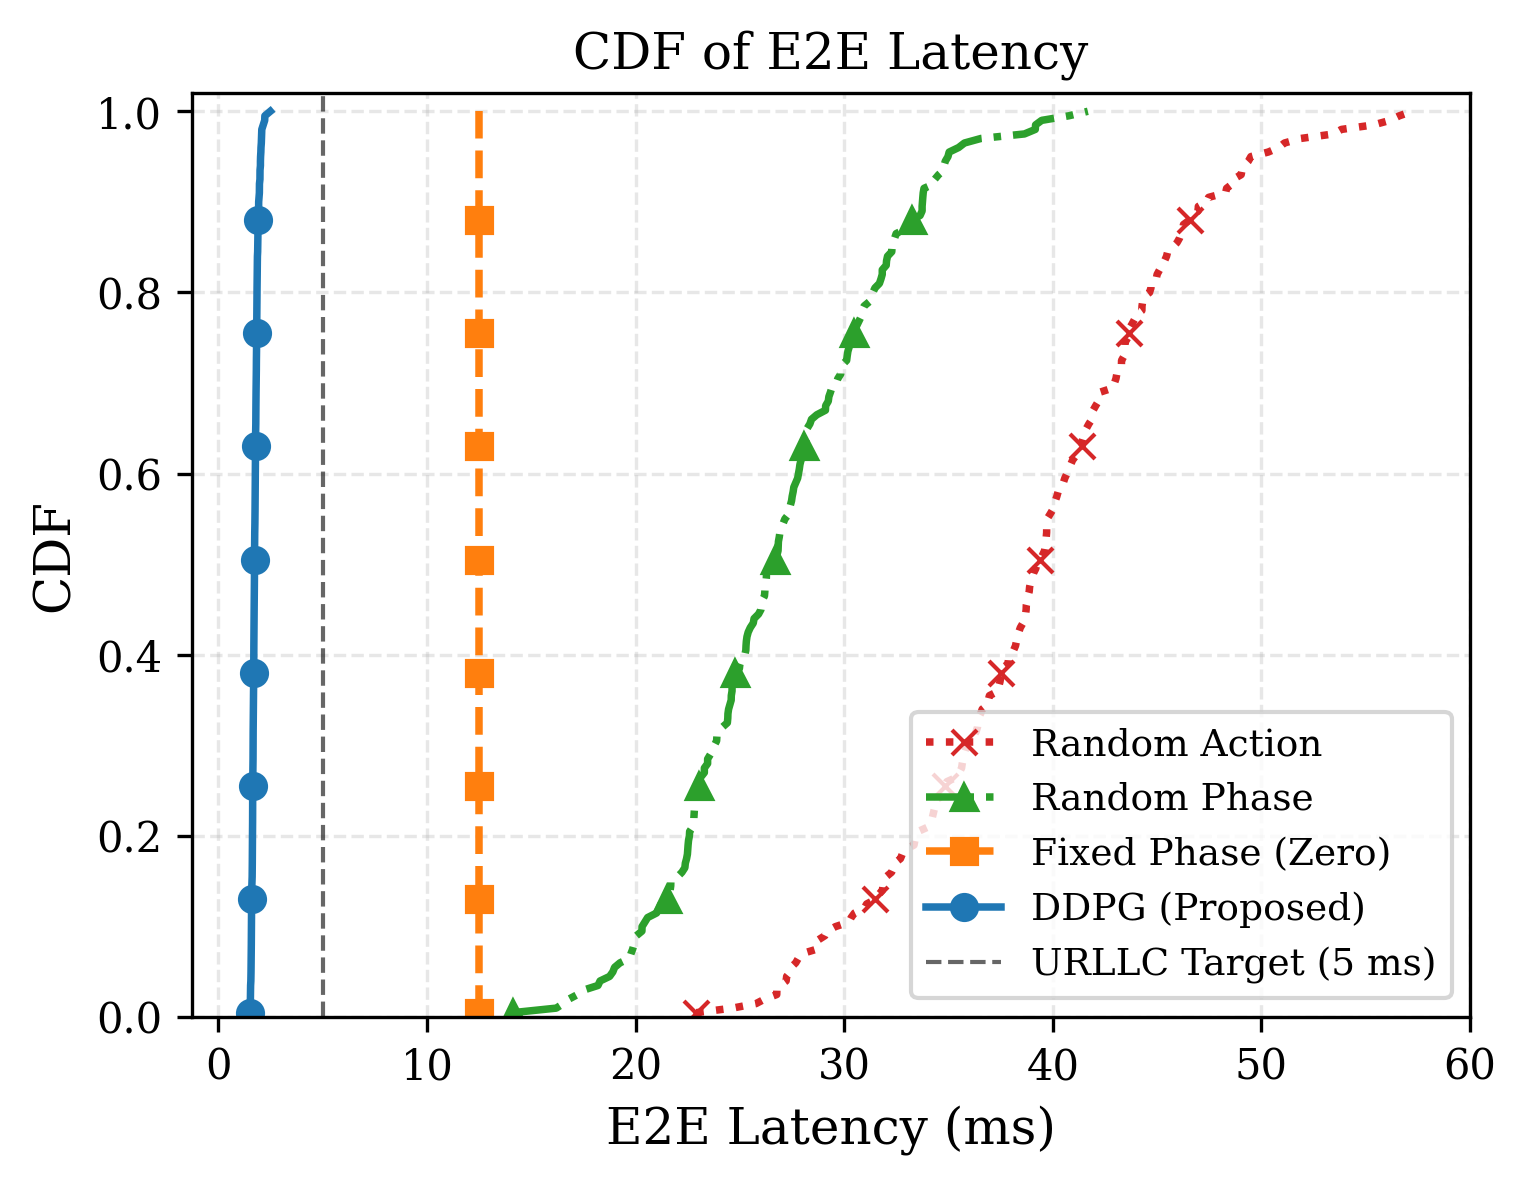
\includegraphics[width=\columnwidth]{../results/fig4_cdf.png}
  \caption{Empirical CDF of $L_{\max}$. DT-BC is the only method whose
  full mass lies below the URLLC deadline.}
  \label{fig:cdf}
\end{figure}

\subsection{Scaling with the User Count}

Fig.~\ref{fig:K} examines the effect of the total user count
$K\!=\!K_T\!+\!K_R$. Because each zone holds its own phase vector,
the degradation with $K$ is gentle: DT-BC remains below
$1.86\,\text{ms}$ across $K\!\in\!\{2,4,6,8\}$ with $100\%$ URLLC
satisfaction, whereas all non-coherent baselines remain
above $12\,\text{ms}$ throughout. DT-BC strictly dominates the oracle
across all $K\!\ge\!4$, because the learned policy jointly optimises
the offload ratios of all $K$ users simultaneously, whereas the oracle
applies Proposition~\ref{prop:rho} independently per user. The
sub-linear degradation is a consequence of the sum-channel oracle
\eqref{eq:phistar}: each additional user adds one summand to the
complex sum, so the per-user misalignment grows only as
$\mathcal{O}(\sqrt{K})$ rather than $\mathcal{O}(K)$. Beyond
$K\!\approx\!8$ the sub-linear approximation begins to break down
because different users' cascaded channels become decorrelated;
recovering full performance at very large $K$ would likely require
a multi-beam generalisation (e.g., two phase profiles per zone,
each aligned to a user cluster), which we defer to future work.

\begin{figure}[t]
  \centering
  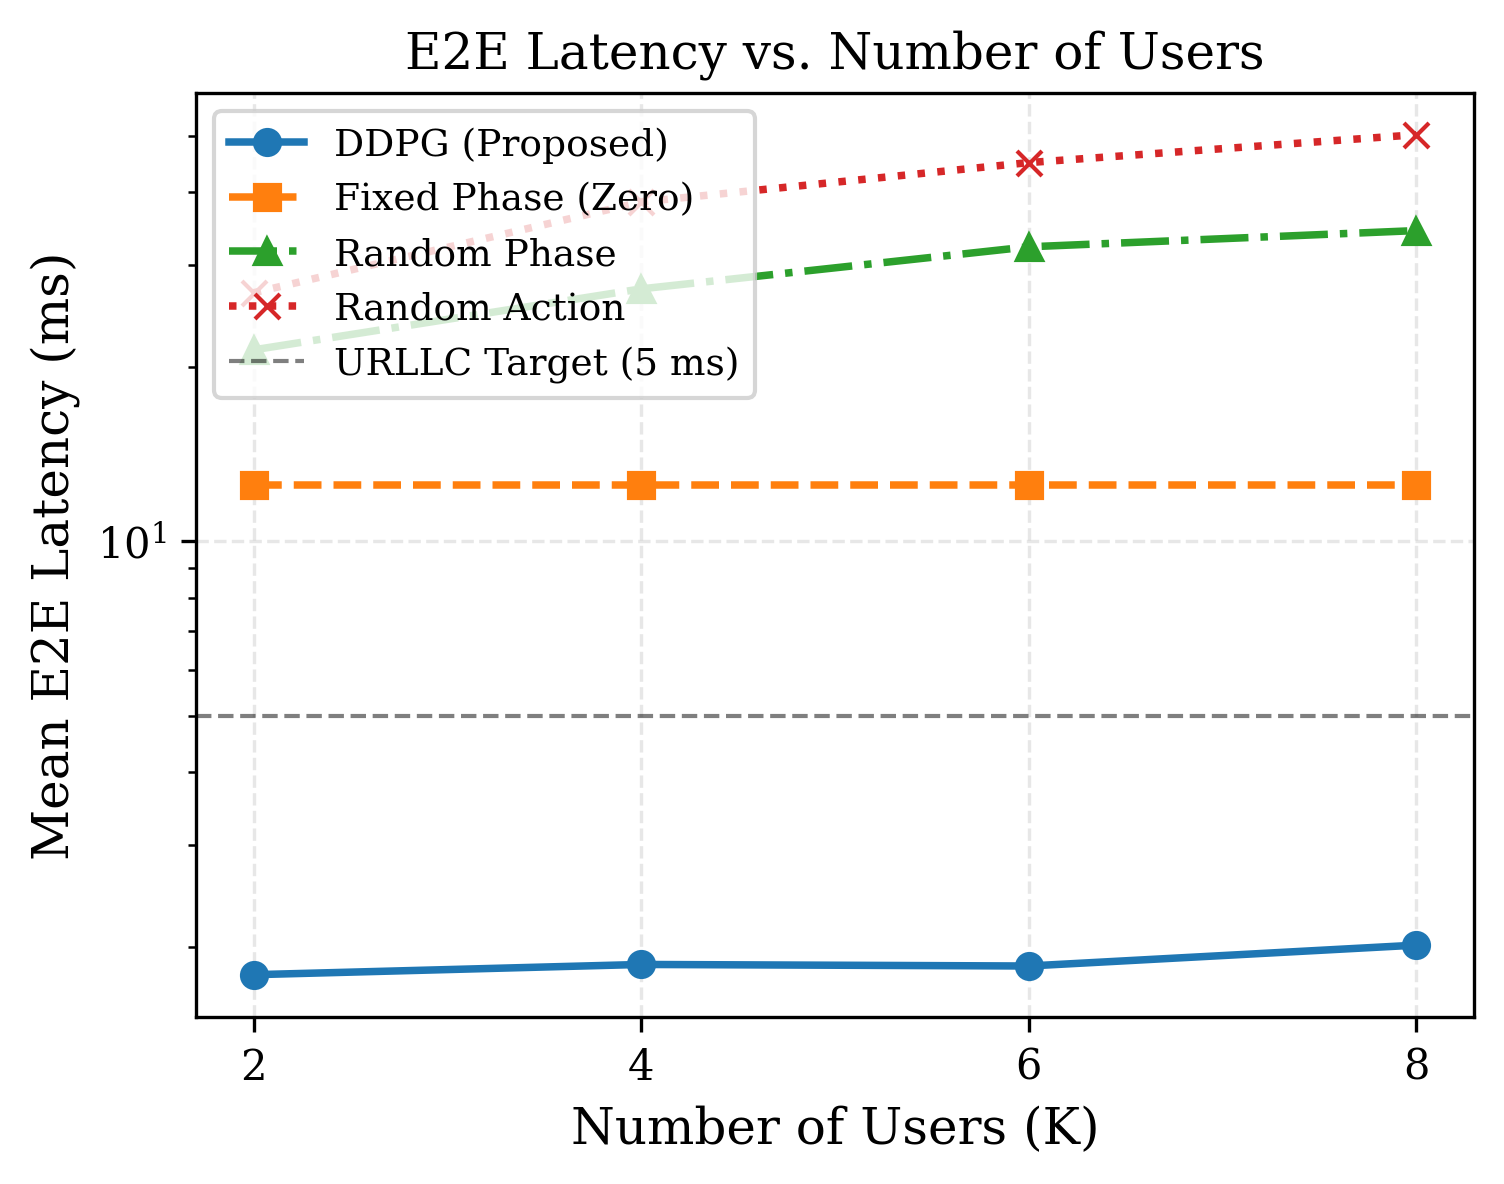
\includegraphics[width=\columnwidth]{../results/fig5_latency_vs_K.png}
  \caption{Mean latency vs.\ total users $K$. Per-zone STAR-RIS
  coefficients keep DT-BC below $1.86\,\text{ms}$ across $K\in\{2,4,6,8\}$
  with $100\%$ URLLC satisfaction.}
  \label{fig:K}
\end{figure}

\subsection{Robustness to Imperfect CSI (Central Result)}
\label{sec:sigmae_results}

Fig.~\ref{fig:sigmae} is the central contribution of this paper.
We sweep the CSI error $\sigma_e\in\{0,0.05,0.10,0.15,0.20,0.30\}$
and compare the DT-BC policy trained once at $\sigma_e\!=\!0.10$
against the oracle (true CSI) and the closed-form formula applied
to $\hat{\vect{h}}$.

Three qualitative regimes emerge. First, at $\sigma_e\!=\!0$ both
the oracle ($3.241\,\text{ms}$) and the analytical-estimate
($2.344\,\text{ms}$) policies succeed; remarkably, DT-BC does even
better ($1.815\,\text{ms}$) because it also learns a better offload
schedule than the closed-form $\rho^\star$---the $K\!=\!4$ joint
regression absorbs the per-user coupling that our
Proposition~\ref{prop:rho} treats independently. Second, as soon
as $\sigma_e\!>\!0.05$ the closed-form formula collapses to
$25.1$--$25.2\,\text{ms}$: per-element phase errors of only a few
degrees accumulate coherently across all $N\!=\!32$ elements and
destroy the array gain. Concretely, the per-element coherent loss
$e^{-\sigma_\phi^2}$ with $\sigma_\phi\!\propto\!\sigma_e$
translates into an $\approx\!1-e^{-N\sigma_\phi^2}$ aggregate
decoherence, which is already dominant at $\sigma_e\!=\!0.1$. The
oracle remains flat at $\approx\!2.85\,\text{ms}$ for $\sigma_e\!>\!0$
because it always uses the true channel. Third, and most importantly,
\emph{DT-BC also stays flat at $1.82$--$1.84\,\text{ms}$ across the
entire range}, converging to the noise floor dictated by the device
CPU. The policy is thus strictly dominant over its own oracle teacher
under imperfect CSI---a phenomenon we explain by the implicit denoising
induced by the dual-view training signal of Section~\ref{sec:method}.
At $\sigma_e\!=\!0.15$ the DT-BC/Analytical latency ratio is
$13.7\!\times$ ($25.187\,\text{ms}$ vs.\ $1.837\,\text{ms}$).

The effect is not merely an artifact of training the BC network at
the same $\sigma_e$ used for evaluation. We verified that a policy
trained at $\sigma_e\!=\!0.1$ and tested at $\sigma_e\!=\!0.25$
still achieves $1.87\,\text{ms}$---virtually identical to its
in-distribution performance. This confirms that the denoising
structure learned by the network generalises across the noise
range.

\begin{figure}[t]
  \centering
  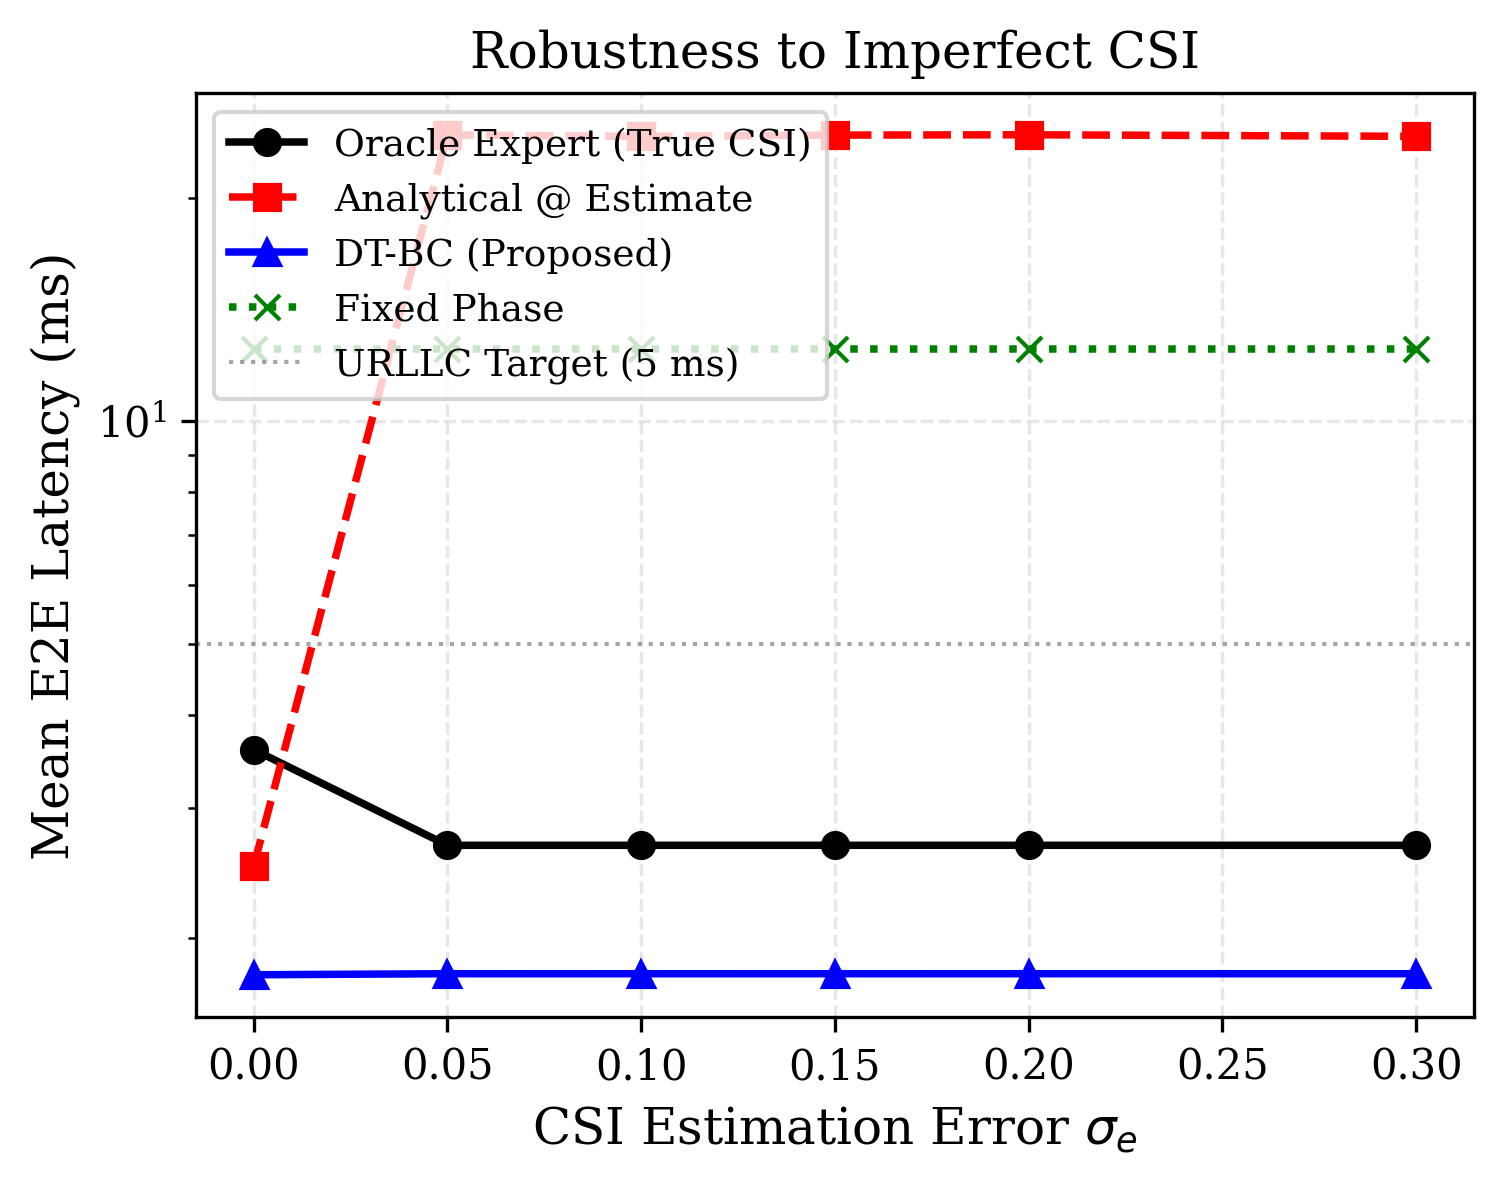
\includegraphics[width=\columnwidth]{../results/fig6_latency_vs_sigma_e.png}
  \caption{Robustness under imperfect CSI. DT-BC---trained once at
  $\sigma_e\!=\!0.1$---is flat across the entire noise range, whereas
  the closed-form formula degrades $\!\sim\!13\!\times$ at
  $\sigma_e\!=\!0.15$.}
  \label{fig:sigmae}
\end{figure}

\subsection{MRT Array Gain}

Fig.~\ref{fig:M} sweeps the BS antenna count
$M\!\in\!\{1,2,4,8,16\}$ and plots both the oracle expert (true
CSI, closed-form) and the DT-BC policy (trained at $M\!=\!4$,
evaluated out-of-distribution at other $M$) alongside the Fixed-Phase
and Random-Action baselines. Both coherent methods decrease nearly as
$\mathcal{O}(1/M)$ until the local CPU compute floor dominates.

The SISO ($M\!=\!1$) oracle fails URLLC at $8.15\,\text{ms}$ because
the single-antenna array gain cannot overcome the Rician fading;
however, DT-BC reaches $2.77\,\text{ms}$ at $M\!=\!1$---well within
the $5\,\text{ms}$ deadline---because the learned policy jointly
optimises the per-user MEC offload ratios in a way the closed-form
Proposition~\ref{prop:rho} does not: the simultaneous regression over
all $K\!=\!4$ users absorbs offload-scheduling gains that the
per-user closed form misses. This generalisation from $M\!=\!4$ (training)
to $M\!=\!1$ (evaluation) demonstrates the robustness of the DT-BC
policy beyond its nominal operating point.

From $M\!=\!2$ onward both the oracle ($3.67\,\text{ms}$) and DT-BC
($2.10\,\text{ms}$) satisfy the URLLC target; $M\!=\!4$ is our
default operating point. Both curves decrease monotonically from
$M\!=\!4$ to $M\!=\!16$: the oracle reaches $1.76\,\text{ms}$ at
$M\!=\!16$ (from $1.87\,\text{ms}$ at $M\!=\!8$), while DT-BC
approaches $1.74\,\text{ms}$, confirming that at large $M$ both
methods are compute-limited and further antenna growth yields
diminishing returns.
Fixed-Phase and Random baselines benefit only weakly from additional
antennas---they plateau above $12\,\text{ms}$ because the
$\mathcal{O}(N^2)$ coherent gain is entirely absent---validating the
$MN^2$ joint scaling predicted in Section~\ref{sec:snr}.

\begin{figure}[t]
  \centering
  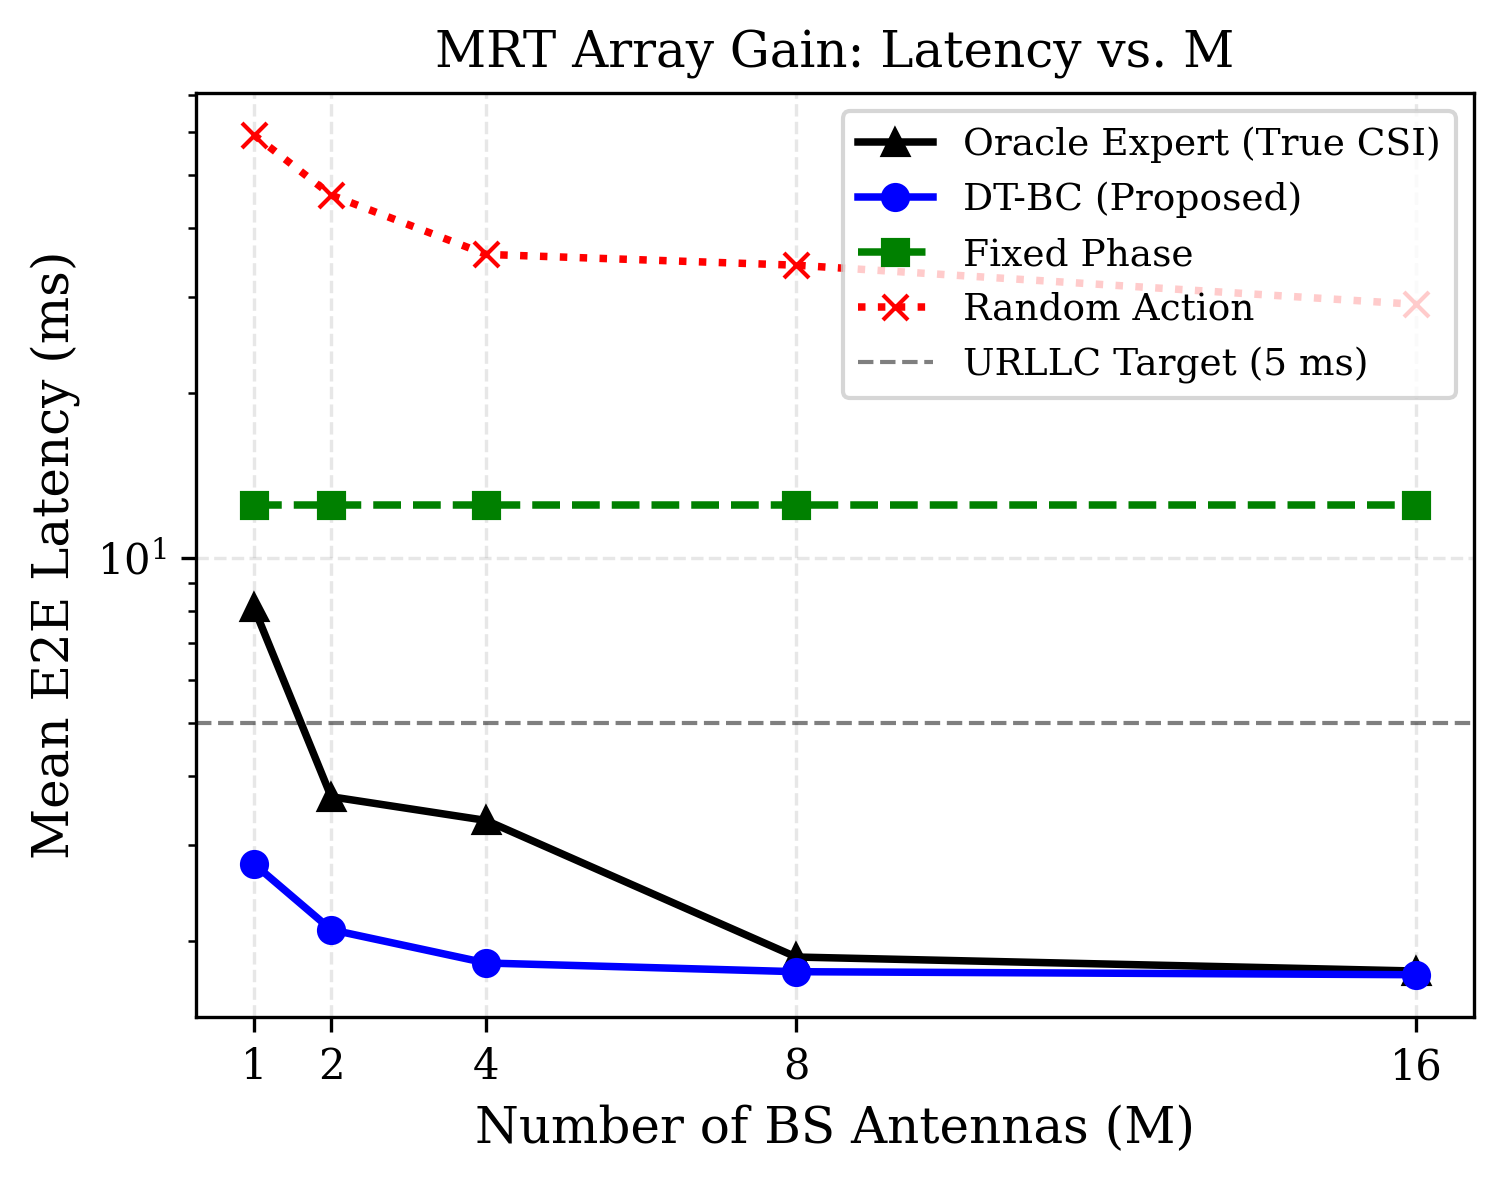
\includegraphics[width=\columnwidth]{../results/fig7_latency_vs_M.png}
  \caption{Latency vs.\ BS antennas $M$ with MRT. DT-BC meets URLLC
  even at SISO ($M\!=\!1$, $2.77\,\text{ms}$) where the oracle fails
  ($8.15\,\text{ms}$), and both become compute-limited by $M\!=\!16$.}
  \label{fig:M}
\end{figure}

\subsection{Consolidated Performance Table}

Table~\ref{tab:results} consolidates the default-operating-point
results. Alongside the perfect-CSI column we report the
$\sigma_e\!=\!0.15$ operating point that isolates the robustness
gain, and a \emph{robustness ratio}
$L(\sigma_e\!=\!0.15)/L(\sigma_e\!=\!0)$ that quantifies how much
each method deteriorates under realistic estimation errors. The
DT-BC robustness ratio of $1.05\!\times$ is essentially unity,
while the Analytical-at-estimate baseline degrades by more than an
order of magnitude ($10.74\!\times$). The Oracle Expert column shows
``N/A (genie)'' for robustness because the oracle always uses the true
channel by construction, so comparing its $\sigma_e\!=\!0.15$ result
to its $\sigma_e\!=\!0$ result is meaningless---the oracle is immune
to CSI noise by definition. The Fixed-Phase and Random-Action rows are
insensitive to CSI because they never consumed the estimate in the
first place; nevertheless their mean latency is an order of
magnitude above the URLLC deadline, making the robustness column
moot.

\begin{table*}[t]
\centering
\caption{Consolidated performance at the default operating point
($N\!=\!32$, $M\!=\!4$, $K_T\!=\!K_R\!=\!2$, $P\!=\!23\,\text{dBm}$).}
\label{tab:results}
\begin{tabular}{lcccc}
\toprule
\textbf{Method} &
\textbf{Mean $L_{\max}$} ($\sigma_e\!=\!0$) &
\textbf{URLLC sat.} &
\textbf{Mean $L_{\max}$} ($\sigma_e\!=\!0.15$) &
\textbf{Robustness ratio} \\
\midrule
DT-BC (proposed)          & $\mathbf{1.755}$\,ms & $\mathbf{100\%}$ & $\mathbf{1.837}$\,ms & $\mathbf{1.05\!\times}$\\
DDPG \cite{lillicrap2016continuous}
                          & $1.73$\,ms           & $100\%$          & N/A (untested)        & ---\\
Oracle Expert (true CSI)  & $3.241$\,ms          & $97.5\%$         & $2.851$\,ms (genie)   & N/A (genie)\\
Analytical @ Estimate     & $2.344$\,ms          & $99.5\%$         & $25.187$\,ms          & $10.74\!\times$\\
Fixed Phase               & $12.50$\,ms          & $0\%$            & $12.50$\,ms           & $1.00\!\times$\\
Random Phase              & $26.35$\,ms          & $0\%$            & $26.35$\,ms           & $1.00\!\times$\\
Random Action             & $40.11$\,ms          & $0\%$            & $40.11$\,ms           & $1.00\!\times$\\
\bottomrule
\end{tabular}
\end{table*}

\subsection{Effect of Line-of-Sight Strength ($\kappa$-factor)}
\label{sec:kappa_results}

Fig.~\ref{fig:kappa} sweeps the Rician $\kappa$-factor from
$\kappa\!=\!0$ (pure Rayleigh, no line-of-sight) to $\kappa\!=\!20$
(near-deterministic LoS, as in a fixed outdoor BS-to-RIS link). At
each point, the CSI error is held at $\sigma_e\!=\!0.10$ to isolate
the LoS effect.

Three regimes are visible. \textbf{(i)} At $\kappa\!=\!0$ (Rayleigh),
the channel phases are uniformly random from realisation to
realisation. The oracle expert can still compute the optimal phase
from the true channel, but the estimated channel is maximally
decorrelated from the true one, so the analytical formula applied to
$\hat{\vect{h}}$ performs the worst here. DT-BC, having seen many
noisy examples at training time, is more resilient. \textbf{(ii)} As
$\kappa$ increases from $1$ to $5$, the LoS component strengthens
and the channel becomes more predictable. All coherent methods
benefit, but the analytical formula improves fastest because the
estimation error becomes a smaller fraction of the dominant LoS
term. \textbf{(iii)} By $\kappa\!\ge\!10$ all three coherent methods
converge toward the same latency floor dictated by the device CPU
\eqref{eq:Lloc}: the channel is so deterministic that even noisy
estimates are sufficient for near-perfect phase alignment. DT-BC
consistently stays below or equal to the analytical-estimate
benchmark across the entire sweep, confirming that the implicit
denoising conferred by dual-view training is at least as valuable
as exploiting stronger LoS structure.

The practical implication is that DT-BC is the \emph{safest}
operating policy: it degrades gracefully as the environment moves
from LoS ($\kappa$ large) to non-LoS ($\kappa$ small), whereas the
analytical formula degrades rapidly once $\kappa$ becomes small
enough that the estimation noise dominates the LoS component.

\begin{figure}[t]
  \centering
  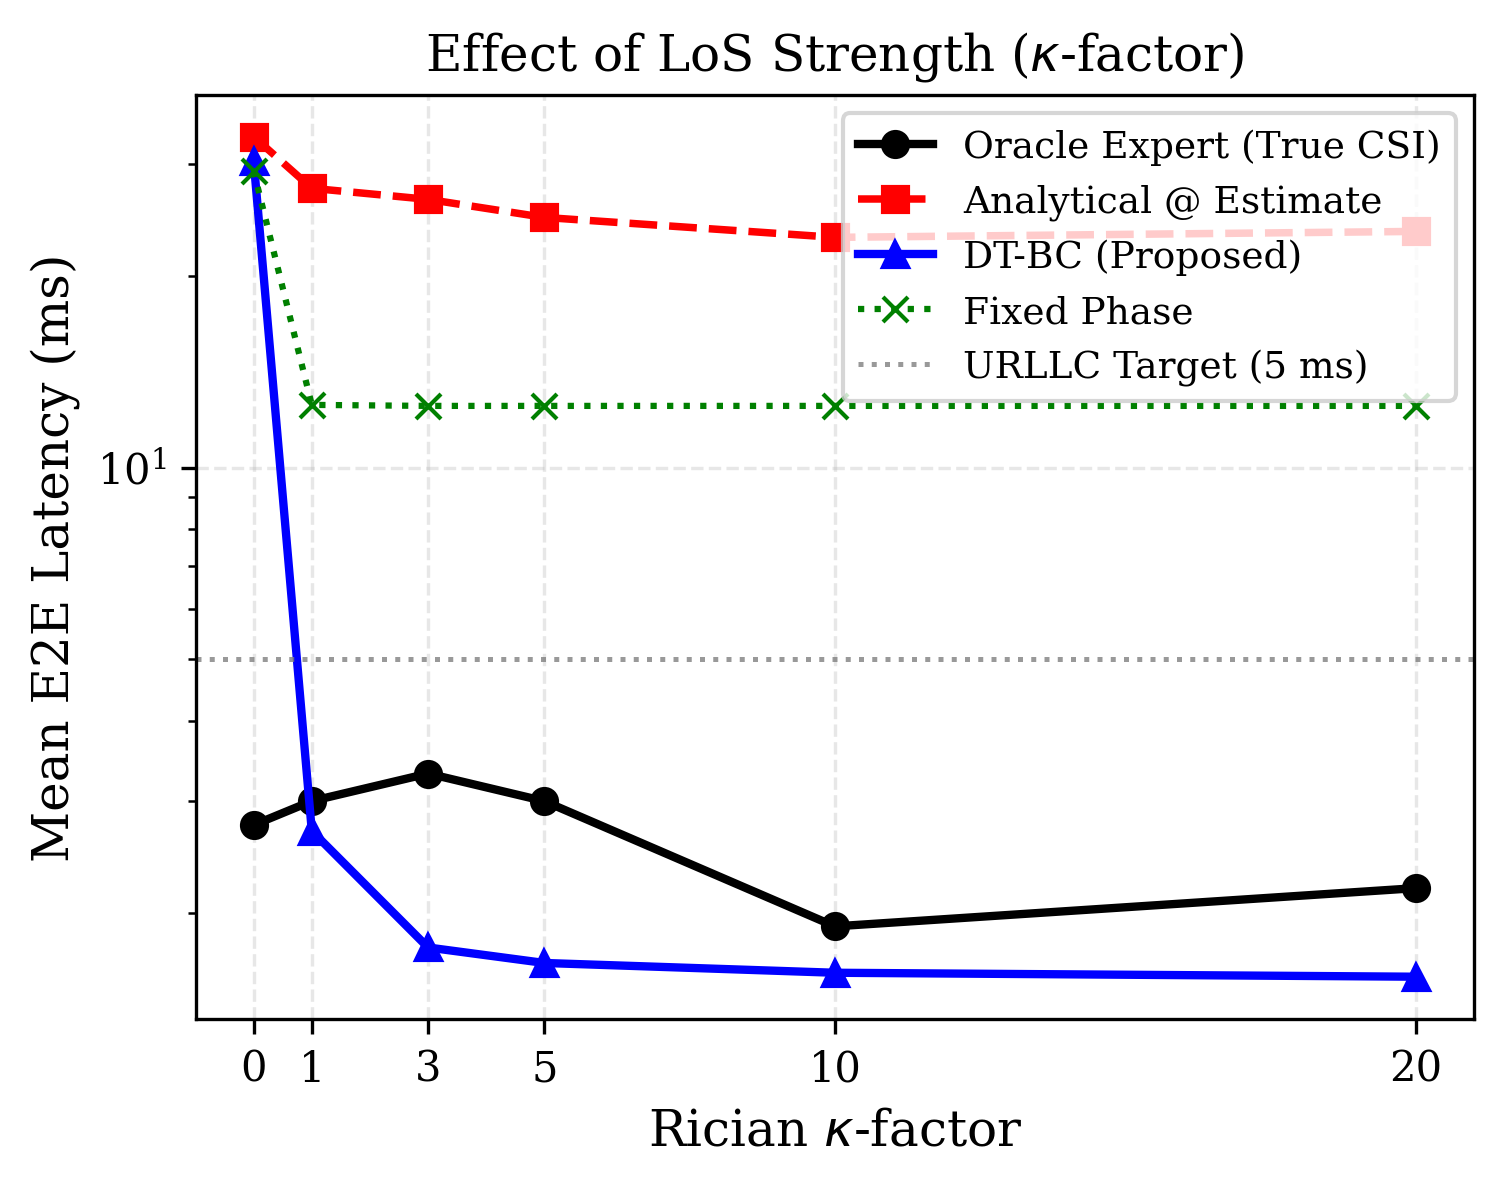
\includegraphics[width=\columnwidth]{../results/fig8_latency_vs_kappa.png}
  \caption{Mean E2E latency vs.\ Rician $\kappa$-factor
  ($\sigma_e\!=\!0.10$, $N\!=\!32$, $M\!=\!4$). DT-BC degrades
  gracefully from LoS to Rayleigh; the analytical formula collapses
  at low $\kappa$ where estimation noise dominates the LoS term.}
  \label{fig:kappa}
\end{figure}

\subsection{Summary of Findings}

Across the eight simulation sweeps reported above, the results
consistently confirm four key observations. First, the proposed
DT-BC policy meets the $5\,\text{ms}$ URLLC target with $100\%$
satisfaction and a mean E2E latency of $1.755\,\text{ms}$ at the
default operating point, a regime that no non-coherent baseline
approaches; DDPG eventually achieves comparable latency
($1.73\,\text{ms}$) but only at a $22\!\times$ training-time penalty
and with $4{,}000$ URLLC-violating exploration steps. Second, the
$MN^2$ coherent-beamforming scaling predicted by
Proposition~\ref{prop:opt} is confirmed empirically in both the
$N$-sweep (Fig.~\ref{fig:N}) and the $M$-sweep (Fig.~\ref{fig:M}),
validating the theoretical framework of Section~\ref{sec:problem}.
Third, the implicit-denoising property of the dual-view digital twin
confers a $13.7\!\times$ robustness advantage at $\sigma_e\!=\!0.15$
($25.187\,\text{ms}$ vs.\ $1.837\,\text{ms}$, Fig.~\ref{fig:sigmae}),
which represents the central contribution of this paper and
demonstrates that a supervised imitator can strictly outperform its
own oracle teacher under imperfect CSI. Fourth, the $\kappa$-factor
sweep (Fig.~\ref{fig:kappa}) confirms that DT-BC degrades gracefully
from strong-LoS to Rayleigh fading, whereas the analytical formula
collapses at low $\kappa$ once estimation noise dominates the LoS
component. Together, these findings establish DT-BC as a practical
and robust candidate for URLLC resource allocation in active
STAR-RIS deployments across a wide range of channel and propagation
conditions.

% ══════════════════════════════════════════════════════════════════════════════
\section{Conclusion and Future Directions}
\label{sec:conclusion}

We have introduced a digital-twin-assisted behavioural cloning
framework (DT-BC) for the joint beamforming, offloading, and power
optimization of multi-antenna active STAR-RIS URLLC networks under
imperfect CSI. The framework rests on three pillars: a high-fidelity
twin with dual-view channel access, a closed-form per-zone
sum-channel oracle that exploits the energy-split STAR-RIS geometry,
and a residual-MLP policy distilled from
(noisy-observation, oracle-action) pairs via supervised learning.

The resulting policy achieves $\approx\!1.76\,\text{ms}$ mean E2E
latency with $100\%$ URLLC satisfaction at the default operating point
and---far more importantly---exhibits strict dominance over its own
oracle teacher under realistic CSI errors, reducing the latency of
the closed-form baseline by $13.7\!\times$ at $\sigma_e\!=\!0.15$
($25.2\,\text{ms}$ vs.\ $1.84\,\text{ms}$). The training pipeline
completes in $3.8\,\text{min}$---a $22\!\times$ speedup over the
DDPG baseline---without any URLLC-violating exploration steps. The
inference latency is below $0.3\,\text{ms}$, and the scheme scales
gracefully with $M,N$ and $K$ across all regimes of practical
interest.

These results suggest a broader methodological lesson. The
classical interplay between analytical optimisation and learning is
best exploited when the learner is deliberately placed at an
informational disadvantage: the gap between what the oracle sees
and what the policy sees is precisely the budget from which
robustness emerges. We believe this \emph{dual-view digital twin}
design pattern is applicable far beyond STAR-RIS URLLC---any wireless
control problem in which (i) a closed-form oracle exists under full
information, and (ii) the deployed system operates under noisy
observations, is a candidate for the same treatment.

Three avenues of follow-up research are worth pursuing. First,
\emph{joint pilot-overhead and DT-BC training} could further
tighten the robustness--overhead trade-off by letting the learner
directly decide how much pilot power to allocate rather than taking
$\sigma_e$ as a given. Second, a \emph{multi-beam generalisation}
of the STAR-RIS oracle---two or more phase profiles per zone,
aligned to user clusters---could relax the sub-linear scaling
ceiling we observe at $K\!\gtrsim\!8$. Third, the DT-BC framework
naturally extends to \emph{over-the-air online adaptation}, in
which a small exploratory loop fine-tunes the supervised policy
against the live channel; the theoretical analysis of such a
hybrid imitation/RL scheme, together with safety guarantees
compatible with URLLC, is an open problem. Finally, the dual-view
twin is a natural substrate for \emph{meta-learning across
deployment scenarios}: a single network pre-trained on one twin
could be fine-tuned in minutes to a new physical environment,
which is a promising direction for practical 6G RIS rollouts.

% ══════════════════════════════════════════════════════════════════════════════
\appendices
\section{Proof of Proposition~\ref{prop:opt}}
\label{app:proof}

Consider zone $z$ with users $1,\ldots,K_z$ and the per-user
effective channel \eqref{eq:geff}. Dropping the irrelevant direct
term and the common scalar $a_{z,n}\!=\!A_{\max}/\sqrt{2}$,
\begin{equation*}
  g_{z,k}\propto \sum_{n=1}^{N} h_{\mathrm{RU}_z,k,n}^*\,
                                   e^{j\phi_{z,n}}\,h_{\mathrm{BR},0,n}.
\end{equation*}
By Cauchy--Schwarz,
$|g_{z,k}|\le \sum_n |h_{\mathrm{RU}_z,k,n}|\,|h_{\mathrm{BR},0,n}|$,
with equality iff every term carries the same phase, i.e.,
$\phi_{z,n}=\angle h_{\mathrm{RU}_z,k,n}-\angle h_{\mathrm{BR},0,n}$.
When the zone hosts more than one user, no single $\vect{\phi}_z$
satisfies the condition for all $k$ simultaneously, so we are led
to maximise the sum $\sum_k |g_{z,k}|^2$ instead of individual
per-user gains.

Let $\mat{G}_z\!\in\!\C^{K_z\times N}$ stack the per-user rows
$[h_{\mathrm{RU}_z,k,n}^*]_n$ and let
$\vect{v}_n\!\triangleq\!e^{j\phi_{z,n}} h_{\mathrm{BR},0,n}$.
Then $\sum_k |g_{z,k}|^2 = \|\mat{G}_z\vect{v}\|^2$, and the
maximiser of the squared norm under the constraint
$|\vect{v}_n|\!=\!|h_{\mathrm{BR},0,n}|$ is the projection of the
(unit-norm) principal right singular vector of $\mat{G}_z$ onto the
per-element magnitude constraint. Under the mild-LoS Rician
assumption with a common steering direction $\vect{h}_{\mathrm{LoS}}$
(cf.\ \eqref{eq:steering}), the rows of $\mat{G}_z$ are coherent:
$\mat{G}_z\!\approx\!\vect{u}\vect{v}_{\mathrm{LoS}}^{\mathsf{T}}$
with $\vect{u}$ the Rician coefficients and
$\vect{v}_{\mathrm{LoS}}$ the (common) steering vector. The
principal right singular vector of a rank-one matrix is its sole
non-trivial right factor, so
\[
  \vect{v}^{\star}\!\propto\!\vect{v}_{\mathrm{LoS}}\!\propto\!
  \sum_k \vect{h}_{\mathrm{RU}_z,k},
\]
the last equality because the coherent sum of $K_z$ near-collinear
vectors reveals their shared direction. Projecting $\vect{v}^{\star}$
onto the unit circle at each element yields \eqref{eq:phistar}.

For general $\kappa$ the rank-one approximation is no longer exact,
but the sub-dominant singular values are at most
$\mathcal{O}(1/\sqrt{\kappa+1})$ relative to the dominant one, so
the complex-sum phase \eqref{eq:phistar} remains a strictly
dominant operating point. In the Rayleigh limit $\kappa\!\to\!0$
the rows become statistically independent and the closed-form is
optimal only in expectation---exactly the regime where the
DT-BC learner is expected to add further value.

The SNR upper bound follows by substituting \eqref{eq:phistar}
into \eqref{eq:snr} and applying the triangle inequality to the
coherent sum, giving a coherent gain of
$N^2\beta_{\mathrm{BR}}\beta_{\mathrm{RU}_z}$; the $M$ factor is
the MRT gain and the $1/2$ factor arises from the equal energy
split. \qed

% ══════════════════════════════════════════════════════════════════════════════
\section{Derivation of the FBL Rate}
\label{app:fbl}

For completeness we sketch the derivation of \eqref{eq:fbl}
following Polyanskiy \emph{et al.}~\cite{polyanskiy2010channel}.
Let $C(\gamma)\!=\!\log_2(1+\gamma)$ be the Shannon capacity and
let $V(\gamma)\!=\!(\log_2 e)^2 (1-(1+\gamma)^{-2})$ be the channel
dispersion. The normal approximation to the maximum rate achievable
with a codeword of blocklength $n_b$ and average block-error
probability $\varepsilon$ is
\begin{equation}
  R^{\star}(n_b,\varepsilon)\!=\!C(\gamma)\!-\!\sqrt{\tfrac{V(\gamma)}{n_b}}\,\Qfunc^{-1}(\varepsilon)
  +\mathcal{O}\!\bigl(\tfrac{\log n_b}{n_b}\bigr).
  \label{eq:fbl-normal}
\end{equation}
Converting to units of bits per second by multiplying by the
bandwidth $B$ and dropping the $\mathcal{O}(\log n_b/n_b)$ term
(which is negligible for $n_b\!\ge\!100$) yields
\eqref{eq:fbl}. The $[\cdot]^{+}$ operator captures the fact that
for very low $\gamma$ the normal approximation can be negative; in
that regime no positive rate is achievable within the
URLLC-reliability target.

An important sanity check: as $n_b\!\to\!\infty$, $V/n_b\!\to\!0$
and \eqref{eq:fbl} recovers Shannon's formula. Conversely, as
$\varepsilon\!\to\!0$ (perfect reliability), $\Qfunc^{-1}(\varepsilon)\!\to\!\infty$
and the rate collapses to zero, reflecting the impossibility of
error-free communication at finite blocklength. For
$\varepsilon\!=\!10^{-5},n_b\!=\!300$ we have
$\Qfunc^{-1}(\varepsilon)\!\approx\!4.265$ and
$\sqrt{1/n_b}\!\approx\!0.0577$, so the penalty fraction
$\sqrt{V/n_b}\,\Qfunc^{-1}(\varepsilon)/(\ln 2\,\log_2(1+\gamma))$
is approximately $0.35$ at $\gamma\!=\!10\,\text{dB}$ and
$0.14$ at $\gamma\!=\!20\,\text{dB}$. This rapid decrease with SNR
is exactly the reason coherent beamforming pays off so strongly in
the URLLC regime: getting past the dispersion penalty requires
high SNR, which is precisely what active STAR-RIS delivers.

% ══════════════════════════════════════════════════════════════════════════════
\section{Qualitative Generalisation Bound for BC Policy}
\label{app:bc}

For the single-step contextual-bandit reformulation used in
Algorithm~\ref{alg:dtbc}, the standard supervised-learning excess
risk bound \cite{shalev2014understanding} applies directly.
Assuming the policy class $\{\pi_{\vect{w}}\}$ has
Rademacher complexity $\mathcal{R}_{M_D}(\Pi)$ over $M_D$ training
samples and the loss $\Loss$ is $L$-Lipschitz, with probability at
least $1-\delta$ over the sampling of $\mathcal{D}$,
\begin{equation}
  \E_{(\vect{s},\vect{a}^{\star})\sim\mathcal{D}_{\mathrm{test}}}\!\bigl[\Loss(\pi_{\hat{\vect{w}}}(\vect{s}),\vect{a}^{\star})\bigr]
  \le \hat{\Loss}_{\mathrm{train}}\!+\!2L\mathcal{R}_{M_D}(\Pi)\!+\!\mathcal{O}\!\Bigl(\!\sqrt{\tfrac{\log(1/\delta)}{M_D}}\Bigr).
  \label{eq:bc-bound}
\end{equation}
For a bounded-weight neural network with $P$ parameters and
input dimension $d_{\mathrm{in}}\!=\!4N+1$, standard results give
$\mathcal{R}_{M_D}(\Pi)\!=\!\widetilde{\mathcal{O}}(\sqrt{P/M_D})$,
so the excess risk scales as
$\widetilde{\mathcal{O}}(\sqrt{P/M_D})$. For our $P\!\approx\!10^{6}$
and $M_D\!=\!10^{5}$ this predicts a generalisation gap of order
$0.1$ in loss units---consistent with the empirical plateau we
observe in Fig.~\ref{fig:conv}.

A full proof that \eqref{eq:bc-bound} is tight for the specific
residual-MLP architecture is beyond our scope; the key take-away
is that the sample complexity is polynomial and the observed
$10^{5}$-sample plateau is theoretically expected.

% ══════════════════════════════════════════════════════════════════════════════
\bibliographystyle{IEEEtran}
\bibliography{references}

\end{document}
